\documentclass{article}

\usepackage{arxiv}

\usepackage[utf8]{inputenc} % allow utf-8 input
\usepackage[T1]{fontenc}    % use 8-bit T1 fonts
\usepackage{lmodern}        % https://github.com/rstudio/rticles/issues/343
\usepackage{hyperref}       % hyperlinks
\usepackage{url}            % simple URL typesetting
\usepackage{booktabs}       % professional-quality tables
\usepackage{amsfonts}       % blackboard math symbols
\usepackage{nicefrac}       % compact symbols for 1/2, etc.
\usepackage{microtype}      % microtypography
\usepackage{graphicx}

\title{Unveiling Color Dynamics in Andy Warhol's ``Shot Marilyns'': A
Study on Visual Variations and Perception}

\author{
    Erick S. Arenas V
   \\
    Department of Statistics \\
    University of California, Davis \\
  Davis, CA 95616 \\
  \texttt{\href{mailto:esarenas@ucdavis.edu}{\nolinkurl{esarenas@ucdavis.edu}}} \\
   \And
    Weilin Cheng
   \\
    Department of Statistics \\
    University of California, Davis \\
  Davis, CA 95616 \\
  \texttt{\href{mailto:wncheng@ucdavis.edu}{\nolinkurl{wncheng@ucdavis.edu}}} \\
   \And
    Hengyuan Liu
   \\
    Department of Statistics \\
    University of California, Los Angeles \\
  Los Angeles, CA 90095 \\
  \texttt{\href{mailto:hengyuanliu@g.ucla.edu}{\nolinkurl{hengyuanliu@g.ucla.edu}}} \\
   \And
    Xinhui Luo
   \\
    Department of Statistics \\
    Tufts University \\
  Boston, MA 02155 \\
  \texttt{\href{mailto:xinhui.luo@tufts.edu}{\nolinkurl{xinhui.luo@tufts.edu}}} \\
   \And
    Kathy Mo
   \\
    Department of Statistics \\
    University of California, Los Angeles \\
  Los Angeles, CA 90095 \\
  \texttt{\href{mailto:kathymo24@g.ucla.edu}{\nolinkurl{kathymo24@g.ucla.edu}}} \\
   \And
    Li Yuan
   \\
    Department of Computer Science \\
    Swiss Federal Institute of Technology, Zurich \\
  8092 Zurich, Switzerland \\
  \texttt{\href{mailto:xxxx@ethz.ch}{\nolinkurl{xxxx@ethz.ch}}} \\
  }


% tightlist command for lists without linebreak
\providecommand{\tightlist}{%
  \setlength{\itemsep}{0pt}\setlength{\parskip}{0pt}}



\usepackage{amsmath}
\usepackage{graphicx}
\usepackage{subcaption}
\begin{document}
\maketitle


\begin{abstract}
This study delves into the comparative analysis of five distinct
versions of Andy Warhol's ``Shot Marilyns,'' focusing on the intricacies
of their color composition and distribution. Employing a range of
analytical methods, including relative conditional entropy, this
research investigates the unique color distributions and interrelations
present in each artwork. Through the clustering of the artworks and the
meticulous examination of specified regions of interest (ROIs)---namely,
the backgrounds, hair, eyeshadow, and faces---we have unearthed profound
insights into the constructional variances and similarities among the
images. Our findings reveal that the presupposed uniformity in the
coloration of certain elements stands contradicted, thereby underscoring
the complexity and illusionary nature of color perception in visual art.
\end{abstract}

\keywords{
    shot marilyns
   \and
    marilyn monroe
   \and
    andy warhol
   \and
    region of interest
   \and
    python
  }

\hypertarget{introduction}{%
\section{Introduction}\label{introduction}}

``Shot Marilyns,'' an illustrious artwork by the American artist Andy
Warhol, stands as a testament to his exploration of celebrity culture
and the commodification of images. Created in 1964, this series features
multiple depictions of Marilyn Monroe, crafted in the wake of her
untimely demise, thereby immortalizing her status as a cultural icon.
Warhol's fascination with fame, consumerism, and the media's influence
on societal perceptions is evident in his innovative use of silkscreen
printing. This technique, adopted in August 1962, facilitated a
production-line approach in art-making, enabling Warhol to replicate
images with minor variations. The ``Shot Marilyns'' series, inspired by
Monroe's death in the same year, utilized this method to produce
screenprints of her image, employing photo stencils and a palette of
vibrant inks to transfer her likeness onto canvas. This body of work
underscores Warhol's endeavor to dissect Monroe's persona through
repetitive imagery, each variation rendered in distinct colors and
compositions, allowing for diverse visual interpretations.

The series' repetitive nature serves as a critique of the pervasive
commodification of celebrities, transforming them into ubiquitous
symbols within popular culture. Warhol's strategic use of bright,
contrasting colors aims to encapsulate Monroe's dynamic celebrity
essence, with the vivid hues underscoring her societal allure and
influence. This study seeks to analyze the pixel color distribution in
RGB space across the five ``Shot Marilyns'' images, examining the
interplay between primary colors through relative conditional entropy.
Such an analysis aims to reveal the underlying emotional and symbolic
connotations Warhol might have intended, with color distributions
potentially reflecting varied moods and themes.

In 1964, an intriguing incident further contributed to the series' lore
when Dorothy Podber, a performance artist, mistakenly received
permission from Warhol to ``shoot'' the Marilyns, leading to an act of
literal gunfire that damaged four of the five canvases. This event
birthed the ``Shot Marilyns,'' adding a layer of physical and conceptual
depth to the artwork. Part of our project involves digitally restoring
the ``Blue Marilyn,'' focusing on the gunshot damage, by analyzing and
replicating the surrounding area's color distribution.

\begin{figure}[ht]
  \centering
  \begin{subfigure}{0.3\textwidth}
    \centering
    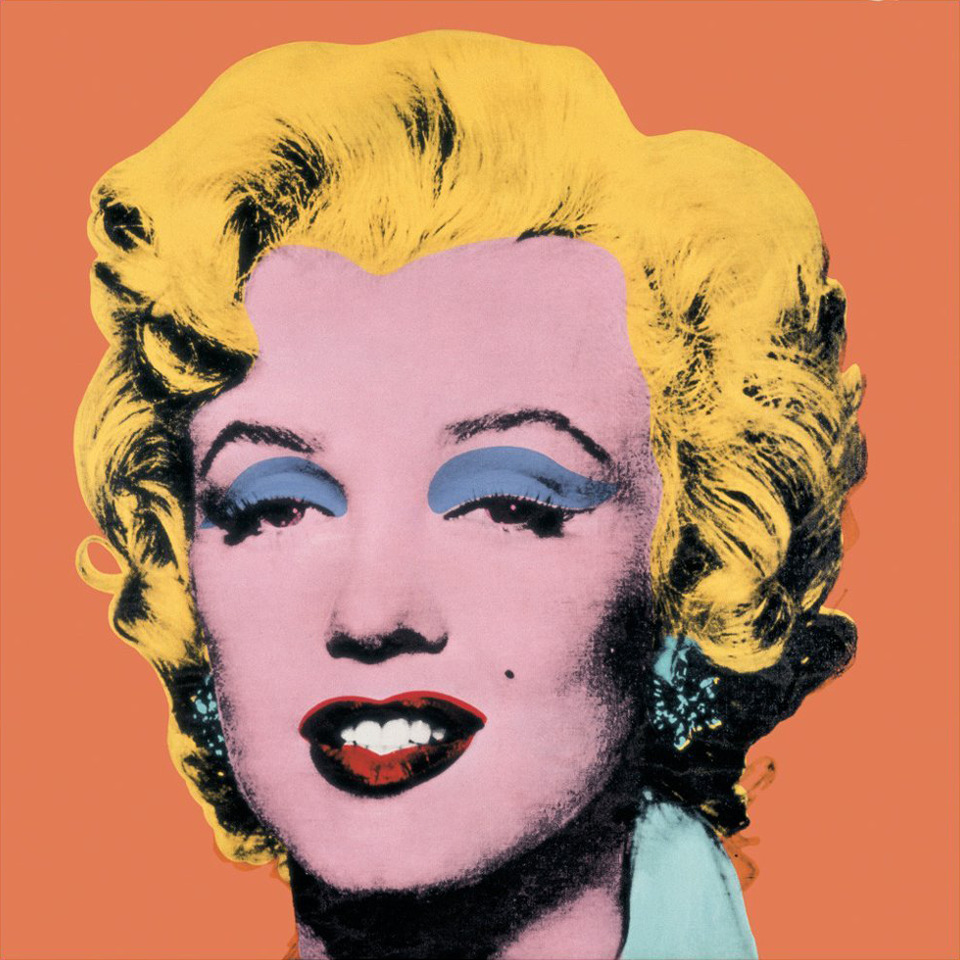
\includegraphics[width=125px]{main_files/figure-latex/1_1_orange_marilyn.jpg}
    \caption{Orange Marilyn}
    \label{fig:1_1_orange_marilyn}
  \end{subfigure}
  \hfill
  \begin{subfigure}{0.3\textwidth}
    \centering
    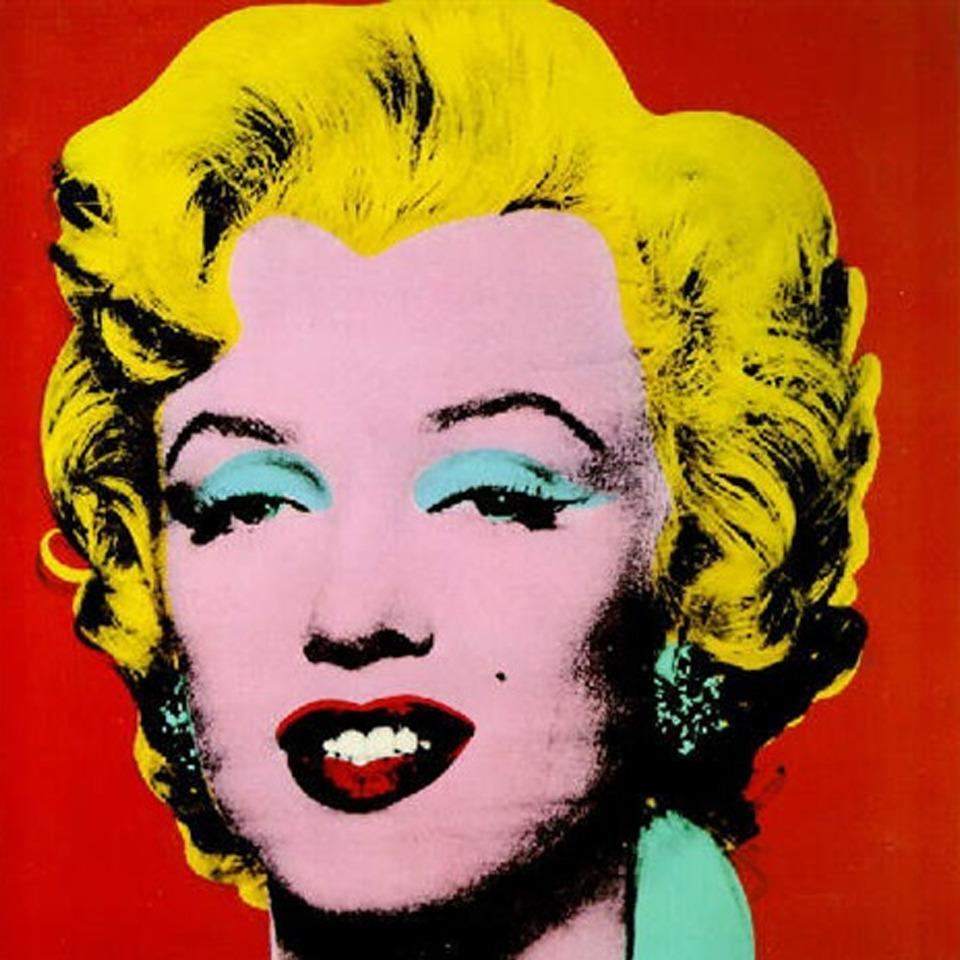
\includegraphics[width=125px]{main_files/figure-latex/1_2_red_marilyn.jpg}
    \caption{Red Marilyn}
    \label{fig:1_2_red_marilyn}
  \end{subfigure}
  \hfill
  \begin{subfigure}{0.3\textwidth}
    \centering
    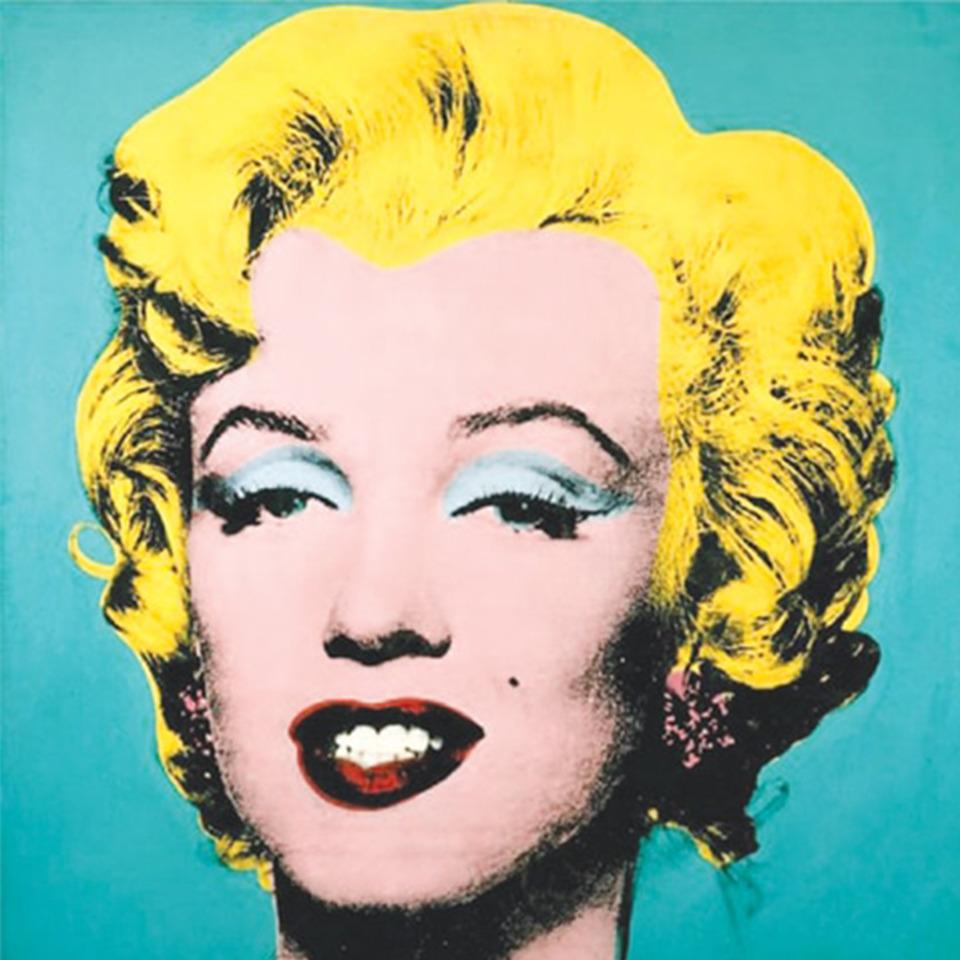
\includegraphics[width=125px]{main_files/figure-latex/1_3_turq_marilyn.jpg}
    \caption{Turquoise Marilyn}
    \label{fig:1_3_turq_marilyn}
  \end{subfigure}

  \vspace{1em}

  \begin{minipage}{0.6\textwidth}
    \centering
    \begin{subfigure}{0.45\textwidth}
      \centering
      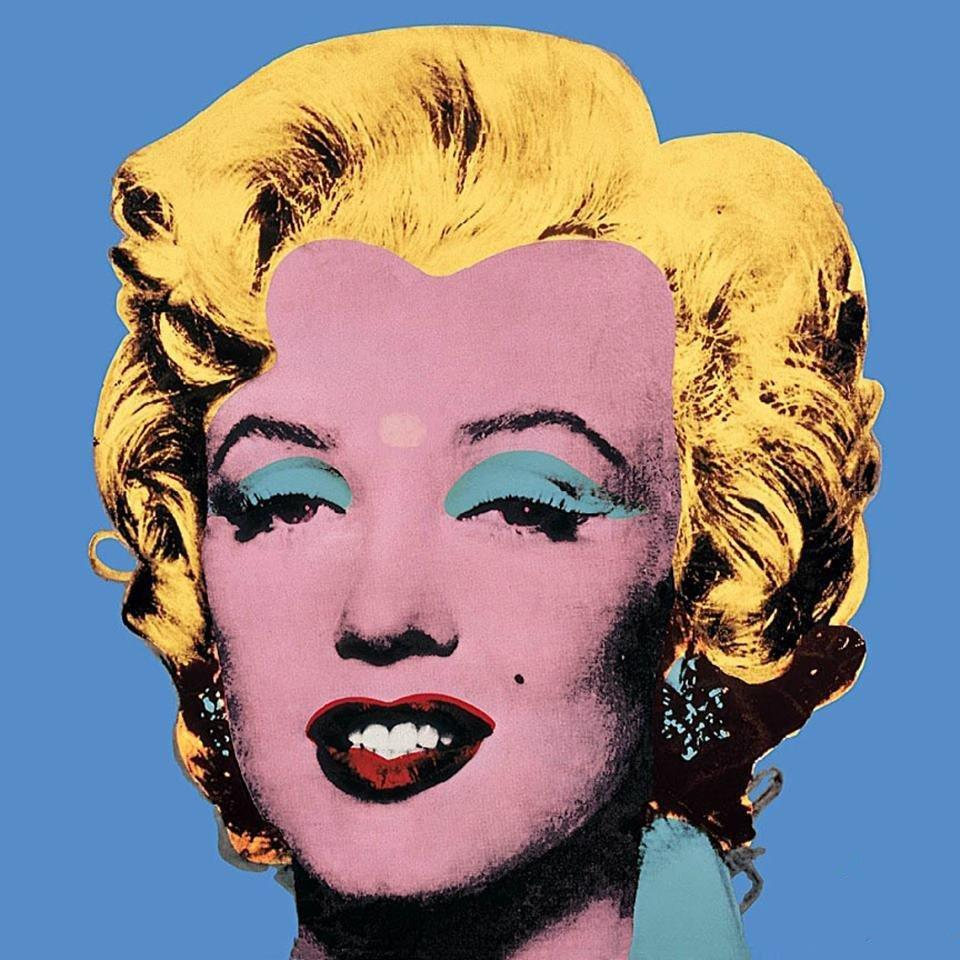
\includegraphics[width=125px]{main_files/figure-latex/1_4_blue_marilyn.jpg}
      \caption{Blue Marilyn}
      \label{fig:1_4_blue_marilyn}
    \end{subfigure}
    \hfill
    \begin{subfigure}{0.45\textwidth}
      \centering
      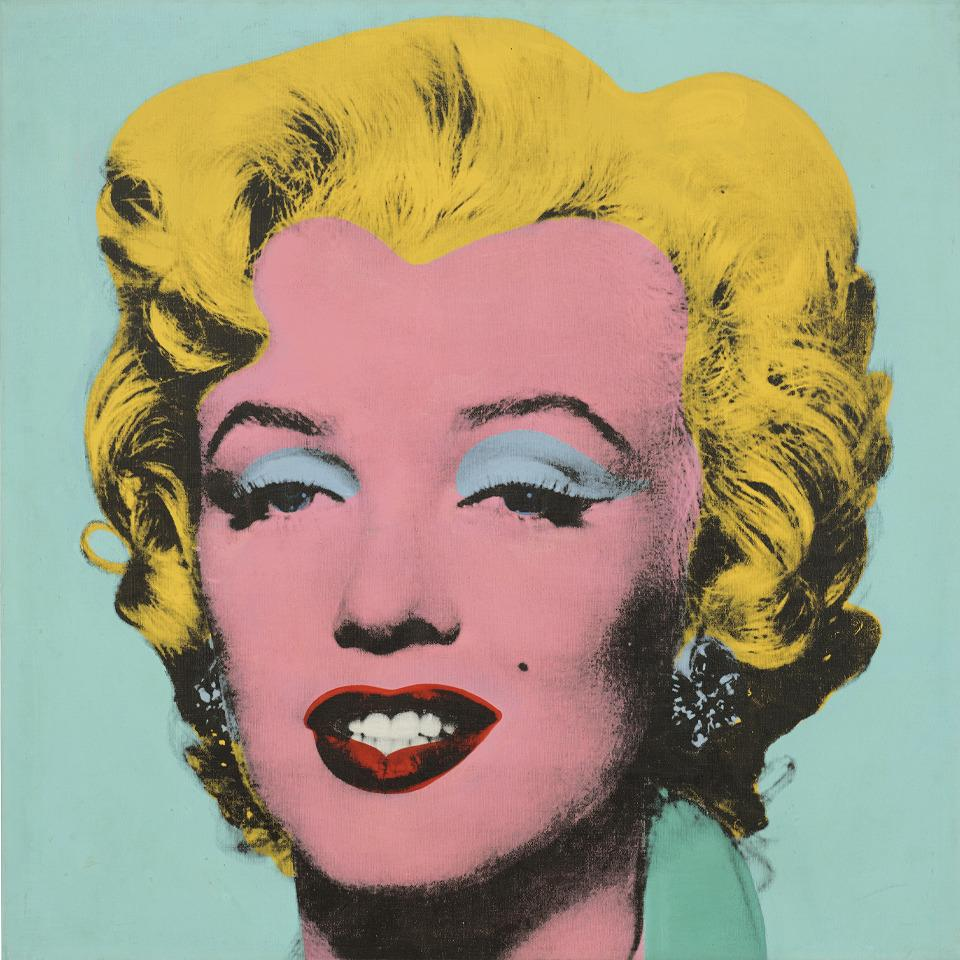
\includegraphics[width=125px]{main_files/figure-latex/1_5_eggblue_marilyn.jpg}
      \caption{Eggblue Marilyn}
      \label{fig:1_5_eggblue_marilyn}
    \end{subfigure}
  \end{minipage}

  \caption{Different color variations of Marilyn Monroe}
  \label{fig:marilyn_variations}
\end{figure}

\hypertarget{methods}{%
\section{Methods}\label{methods}}

An image comprises pixels, with each pixel containing three color
components: Red (R), Green (G), and Blue (B), denoted as (R, G, B)
respectively. These components define the intensity of the respective
colors, with each component represented by an integer value within the
range of {[}0, 255{]} in the RGB color space. Therefore, each color
component is a discrete variable capable of assuming 256 distinct
values. In the equations below, \(Y=y\) or \(X=x\) can be selected from
any of the three color components, R, G, or B.

\hypertarget{entropy-calculation}{%
\subsection{Entropy Calculation}\label{entropy-calculation}}

The probability of a specific color component, \(P(Y=y)\), is determined
by dividing the number of pixels with color coordinates corresponding to
that component by the total number of color components in the entire
image. The following equations illustrate the calculation of entropy,
conditional entropy, and relative conditional entropy

The entropy of a color component \(Y\) is defined as:

\begin{equation}
    H(Y) = - \sum_{y=0}^{255} P(Y = y) \cdot \log(P(Y = y))
\end{equation}

The conditional entropy of \(Y\) given \(X\) is given by:

\begin{equation}
    H(Y|X) = \sum_{x=0}^{255} P(X = x) \cdot H(Y|X = x) = - \sum_{x=0}^{255} \sum_{y=0}^{255} P(X = x, Y = y) \log_2 \left(\frac{P(X = x, Y = y)}{P(X = x)}\right)
\end{equation}

The relative conditional entropy is calculated using the following
formula:

\begin{equation}
    HR(X|Y) = \frac{H(X|Y)}{H(X)}
\end{equation}

\hypertarget{k-means-clustering-analysis}{%
\subsection{K-Means Clustering
Analysis}\label{k-means-clustering-analysis}}

In the clustering analysis, we applied K-Means clustering to analyze the
color dynamics in Andy Warhol's ``Shot Marilyns'' series. For each
image, we performed K-Means clustering using the sklearn library,
specifying the number of clusters (n\_clusters) as 15, the
initialization method (init) as ``k-means++''{[} {]}.(Benefits of using
k-means++) The clustering algorithm grouped pixels into clusters based
on their RGB values, effectively identifying the predominant color in
each image. This method allowed us to quantify and visualize the
distribution of colors, revealing the underlying color patterns and
variations within the artworks. The resulting clusters were then
analyzed to understand the prominence of specific colors across the
series, as depicted in the corresponding bar charts and ribbons. These
visualizations highlight the distinctive color schemes employed by
Warhol, providing insights into his artistic technique and color usage.

\hypertarget{roi-extraction}{%
\subsection{ROI Extraction}\label{roi-extraction}}

In our study of ROI analysis, we employed a method to ROI from the
images in the ``Shot Marilyns'' series include background, hair,
eyeshadow and face. This process involved converting the images to HSV
color space to better identify and segment specific color ranges. We
determined the minimum and maximum HSV values within selected image
regions manually. These values were used to create a color mask, which
isolated the target color regions. The masked image was then processed
to remove unwanted areas, and the resulting ROI was saved and analyzed.
This method enabled us to focus on specific color features in the
artwork, providing detailed insights into Warhol's color use and
variations.

\hypertarget{k-nearest-neighbors-repair}{%
\subsection{K-Nearest Neighbors
Repair}\label{k-nearest-neighbors-repair}}

To address the damaged sections of the ``Blue Marilyn'' image, we
employed K-Nearest Neighbors (KNN) regression for image repair. This
method involves identifying the coordinates of the damaged pixels and
using the surrounding undamaged pixels to predict their values. The KNN
regression model, with a specified number of neighbors, was trained on
the undamaged pixels' RGB values. The model then predicted the RGB
values for the damaged pixels, effectively restoring the affected area.
This approach allowed us to maintain the image's visual consistency by
leveraging the spatial color information of the undamaged regions. The
repaired images were subsequently saved and analyzed to ensure the
accuracy and aesthetic integrity of the restoration process.

\hypertarget{data-description}{%
\section{Data Description}\label{data-description}}

Our study utilized a dataset comprising five images, each retrieved via
URL links provided by ``The Interior Review'' website {[}1{]}. The
images, titled Orange Marilyn, Red Marilyn, Turquoise Marilyn, Blue
Marilyn, and Eggblue Marilyn, are digitally encoded in the RGB color
model. This model synthesizes a spectrum of colors through the additive
mixing of Red, Green, and Blue light. The intensity of each primary
color is quantized into discrete levels, ranging from 0 to 255, offering
a finite palette within this cubic color space. The dimensions of each
image are 960 by 960 pixels, totaling 921,600 unique data points per
image, each specified by a distinct location and its chromatic
composition.

\hypertarget{data-exploration-and-visualization-analysis}{%
\section{Data Exploration and Visualization
Analysis}\label{data-exploration-and-visualization-analysis}}

\begin{figure}[ht]
  \centering
  \begin{subfigure}{0.3\textwidth}
    \centering
    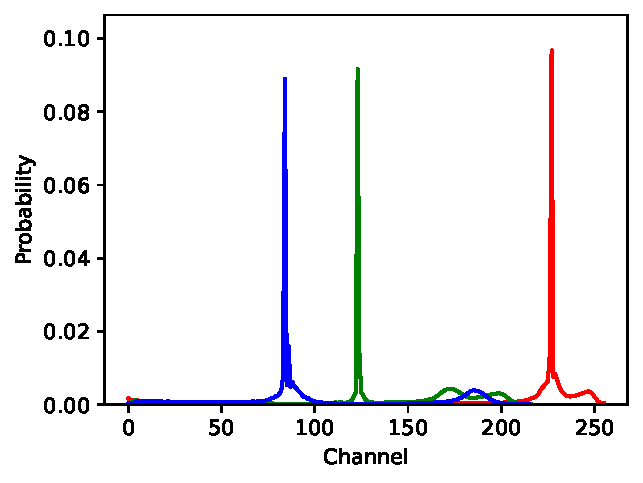
\includegraphics[width=125px]{main_files/figure-latex/2_1_orange_marilyn_dist.pdf}
    \caption{Orange Marilyn RGB Distributions}
    \label{fig:2_1_orange_marilyn_dist}
  \end{subfigure}
  \hfill
  \begin{subfigure}{0.3\textwidth}
    \centering
    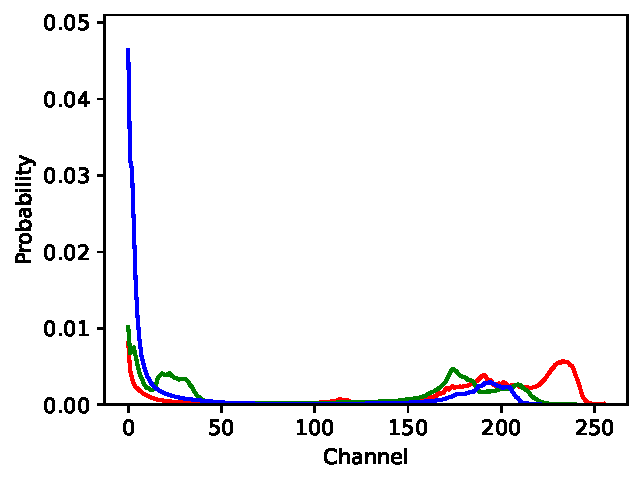
\includegraphics[width=125px]{main_files/figure-latex/2_2_red_marilyn_dist.pdf}
    \caption{Red Marilyn RGB Distributions}
    \label{fig:2_2_red_marilyn_dist}
  \end{subfigure}
  \hfill
  \begin{subfigure}{0.3\textwidth}
    \centering
    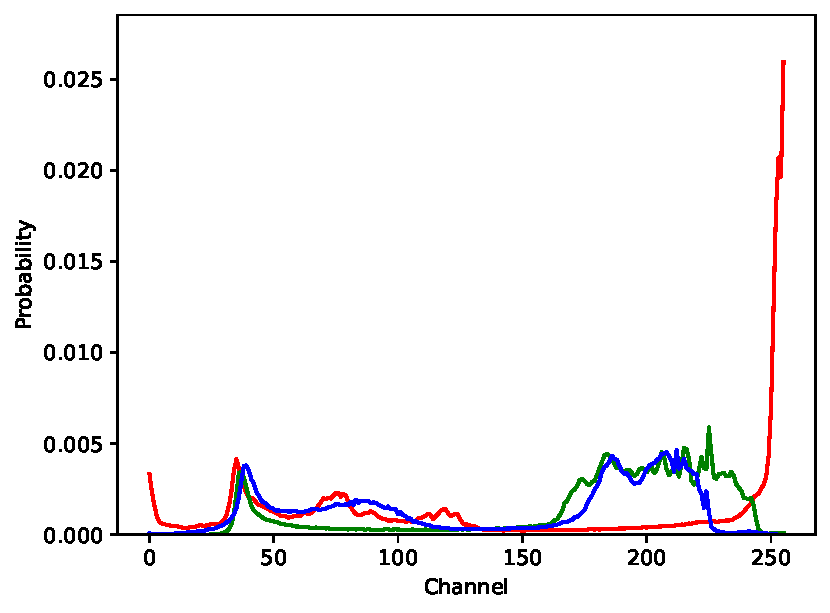
\includegraphics[width=125px]{main_files/figure-latex/2_3_turq_marilyn_dist.pdf}
    \caption{Turquoise Marilyn RGB Distributions}
    \label{fig:2_3_turq_marilyn_dist}
  \end{subfigure}

  \vspace{1em}

  \begin{minipage}{0.6\textwidth}
    \centering
    \begin{subfigure}{0.45\textwidth}
      \centering
      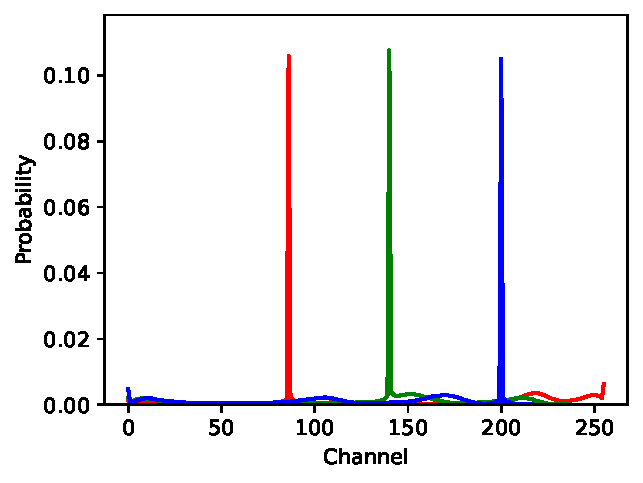
\includegraphics[width=125px]{main_files/figure-latex/2_4_blue_marilyn_dist.pdf}
      \caption{Blue Marilyn RGB Distributions}
      \label{fig:2_4_blue_marilyn_dist}
    \end{subfigure}
    \hfill
    \begin{subfigure}{0.45\textwidth}
      \centering
      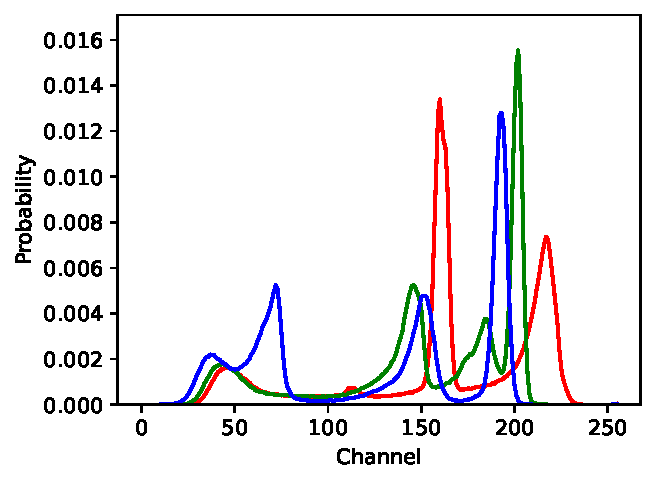
\includegraphics[width=125px]{main_files/figure-latex/2_5_eggblue_marilyn_dist.pdf}
      \caption{Eggblue Marilyn RGB Distributions}
      \label{fig:2_5_eggblue_marilyn_dist}
    \end{subfigure}
  \end{minipage}

  \caption{Distributions of values of Red, Green, and Blue channels for five images with all pixels}
  \label{fig:marilyn_dist}
\end{figure}

Our initial analytical procedure involved scrutinizing the RGB channels
of the images and assessing their distribution profiles. Figure 3
delineates the variation in the red, green, and blue distributions
across the five images. Notably, images (a) and (d) display pronounced
disparities when contrasted with the others. For instance, in the (a)
Orange Marilyn image, the blue channel's most significant probability
density is localized within the {[}50, 100{]} interval, reaching an
estimated 8.5\%. The green channel's peak probability lies between
{[}120, 130{]}, at around 9\%. Similarly, a notable concentration for
blue is observed in the {[}220, 240{]} range with a likelihood of
approximately 10\%.

Intriguingly, image (d) mirrors the (a) Orange Marilyn in terms of green
channel probabilities, predominantly in the {[}120, 130{]} range.
However, it diverges markedly in the red and blue spectra. Image (d)
features a red channel probability apex in the {[}70, 80{]} interval,
representing a 11\% likelihood, while its blue channel's highest
probability is within the {[}190, 210{]} range, also accounting for a
11\% probability. The divergence in the red and blue channel
distributions between images (d) and (a) accentuates their unique
attributes in the collective color distribution.

\begin{figure}[ht]
  \centering
  \begin{subfigure}{0.3\textwidth}
    \centering
    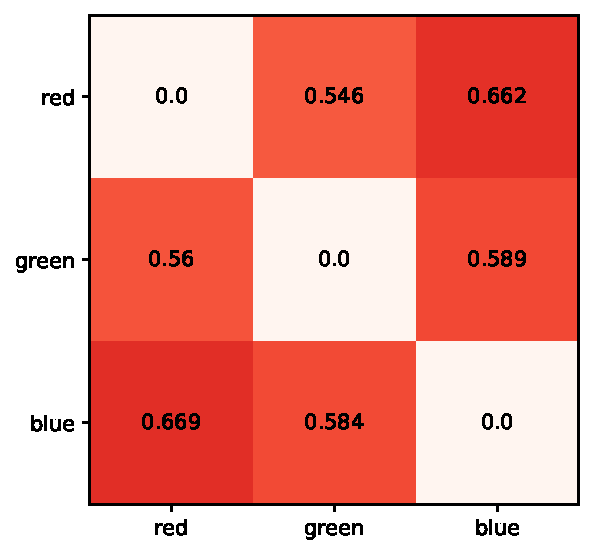
\includegraphics[width=125px]{main_files/figure-latex/3_1_orange_marilyn_entropy.pdf}
    \caption{Orange Marilyn Relative Conditional Entropy}
    \label{fig:3_1_orange_marilyn_entropy}
  \end{subfigure}
  \hfill
  \begin{subfigure}{0.3\textwidth}
    \centering
    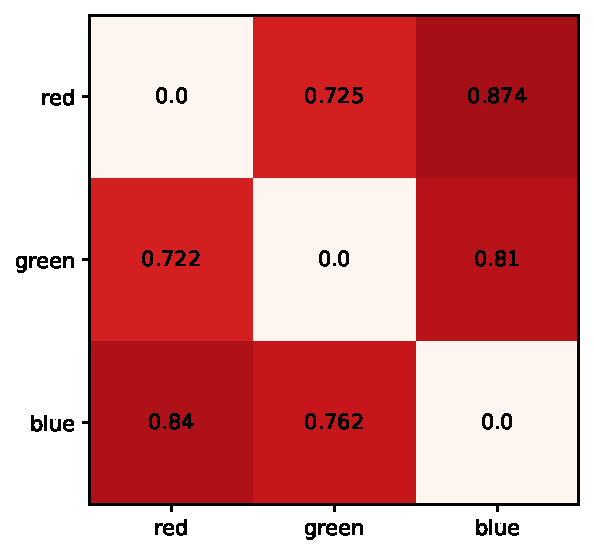
\includegraphics[width=125px]{main_files/figure-latex/3_2_red_marilyn_entropy.pdf}
    \caption{Red Marilyn Relative Conditional Entropy}
    \label{fig:3_2_red_marilyn_entropy}
  \end{subfigure}
  \hfill
  \begin{subfigure}{0.3\textwidth}
    \centering
    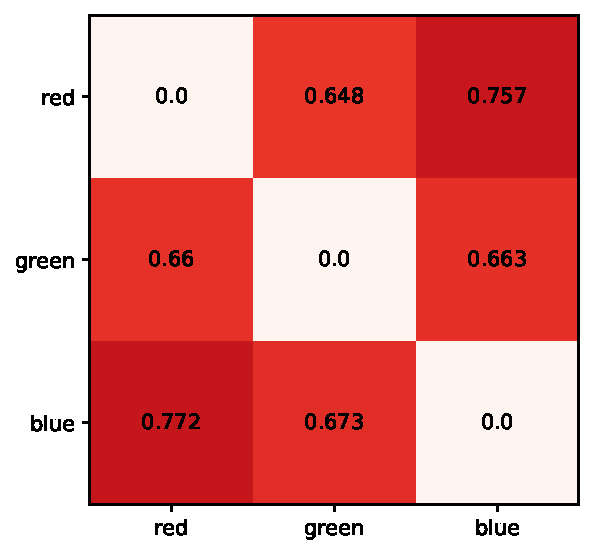
\includegraphics[width=125px]{main_files/figure-latex/3_3_turq_marilyn_entropy.pdf}
    \caption{Turquoise Marilyn Relative Conditional Entropy}
    \label{fig:3_3_turq_marilyn_entropy}
  \end{subfigure}

  \vspace{1em} % Add some vertical space between rows

  \begin{minipage}{0.6\textwidth}
    \centering
    \begin{subfigure}{0.45\textwidth}
      \centering
      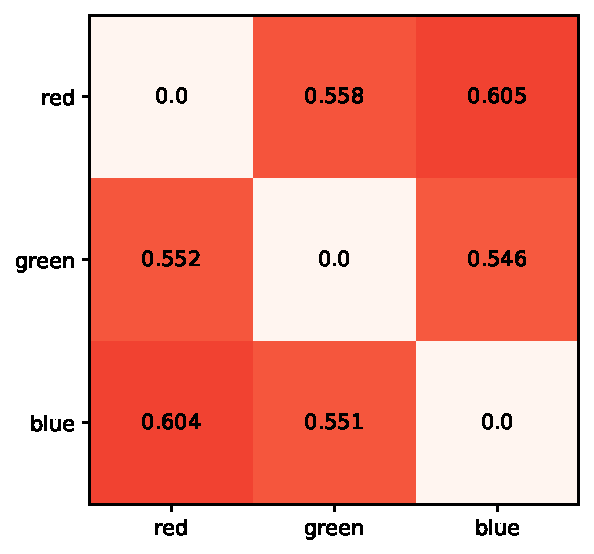
\includegraphics[width=125px]{main_files/figure-latex/3_4_blue_marilyn_entropy.pdf}
      \caption{Blue Marilyn Relative Conditional Entropy}
      \label{fig:3_4_blue_marilyn_entropy}
    \end{subfigure}
    \hfill
    \begin{subfigure}{0.45\textwidth}
      \centering
      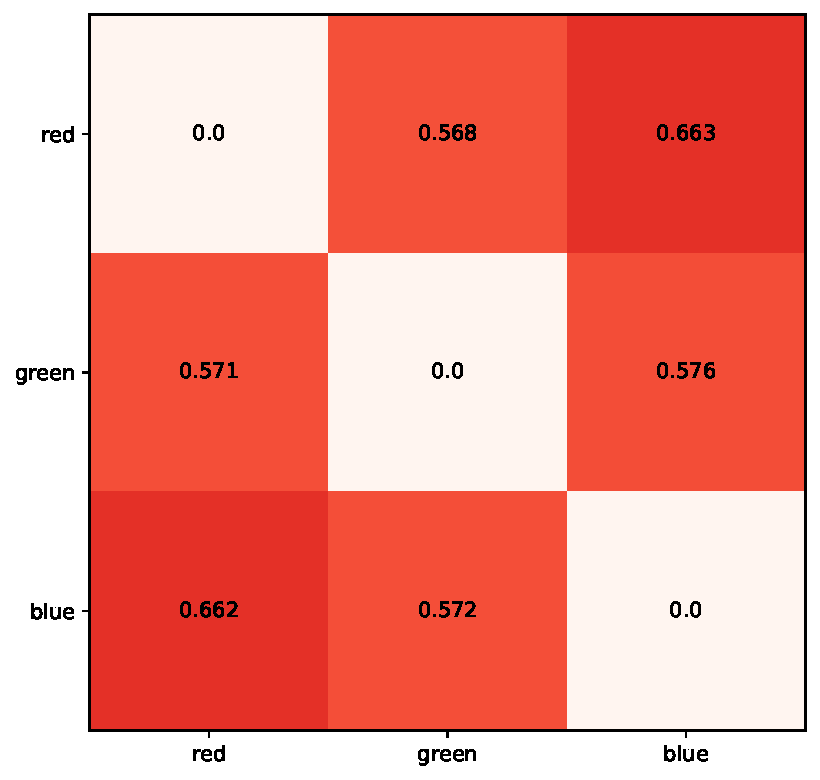
\includegraphics[width=125px]{main_files/figure-latex/3_5_eggblue_marilyn_entropy.pdf}
      \caption{Eggblue Marilyn Relative Conditional Entropy}
      \label{fig:3_5_eggblue_marilyn_entropy}
    \end{subfigure}
  \end{minipage}

  \caption{The relative conditional entropy values among the red, green, and blue coordinates of pixels}
  \label{fig:marilyn_entropy}
\end{figure}

\newpage

After analyzing the RGB distribution of each image, we further
investigated the relationship between pairs of primary colors in the
five images by calculating their relative conditional entropy (HR) (See
Methods 2.1). This metric quantifies the shared information or
dependency between two color channels, with lower HR values indicating
stronger dependencies and higher values suggesting greater independence.
HR ranges from 0 to 1, where 0 signifies complete dependency and 1
represents total independence.

Figure 4 presents the HR values for nine color pairs in each of the five
images: Orange Marilyn, Red Marilyn, Turquoise Marilyn, Blue Marilyn,
and Eggblue Marilyn. As expected, comparing a color to itself yields a
conditional entropy of zero. High HR values for different color pairs
indicate minimal dependency between them. For instance, in the Red
Marilyn image, the HR value for the Red channel relative to the Blue
channel is 0.874, signifying strong independence between the Red and
Blue channels.

\hypertarget{clustering-based-on-whole-images}{%
\section{Clustering based on Whole
Images}\label{clustering-based-on-whole-images}}

Next, we visualized our RGB color data in a 3D space, plotting each
color pair for the entire image. Following figures will present a series
of 3D scatter plots from four distinct angles, with each dot
representing a single pixel. These visualizations illustrate the
distribution of pixel colors in the RGB space, highlighting the
relationships between red, green, and blue coordinates. Viewing the data
from multiple perspectives provides a comprehensive understanding of the
color dynamics, revealing intricate patterns and dependencies within the
images.

\newpage

\begin{figure}[ht]
  \centering
  \begin{subfigure}{0.24\textwidth}
    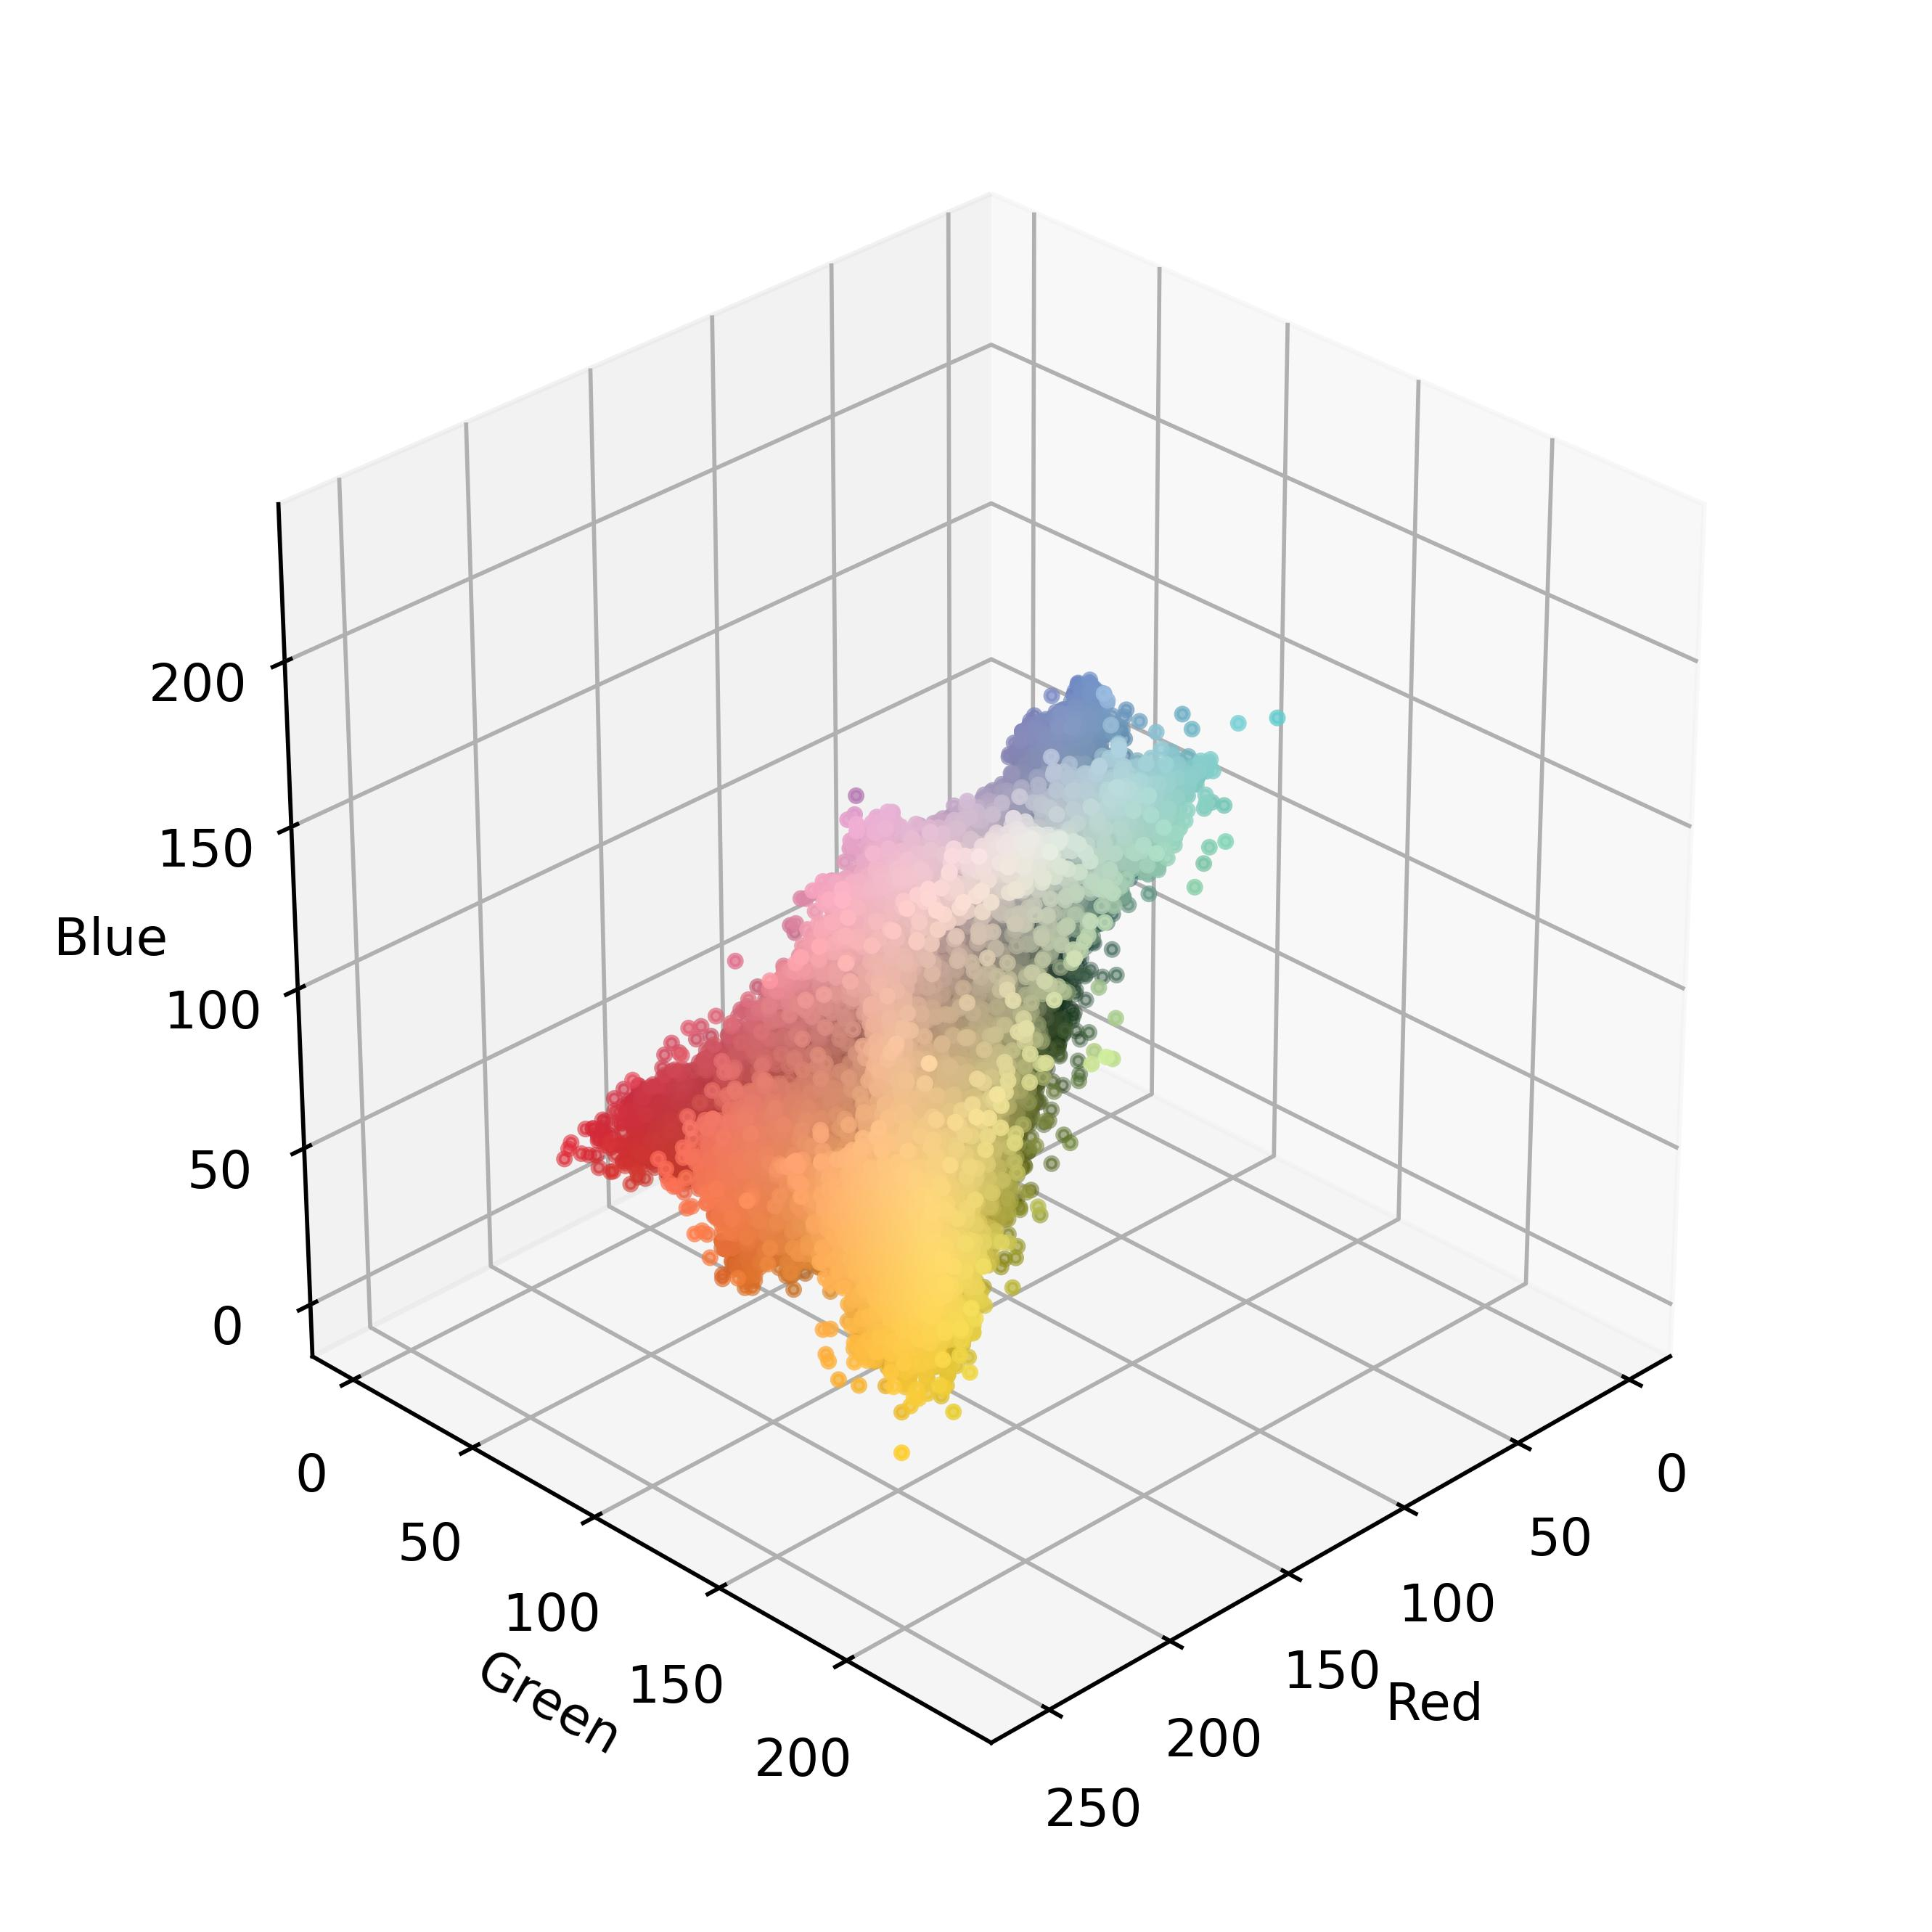
\includegraphics[width=\textwidth]{main_files/figure-latex/4_1_orange_marilyn_original_scatter.jpg}
    \caption{Orange Marilyn RGB Space Angle 1}
    \label{fig:4_1_orange_marilyn_original_scatter}
  \end{subfigure}
  \hfill
  \begin{subfigure}{0.24\textwidth}
    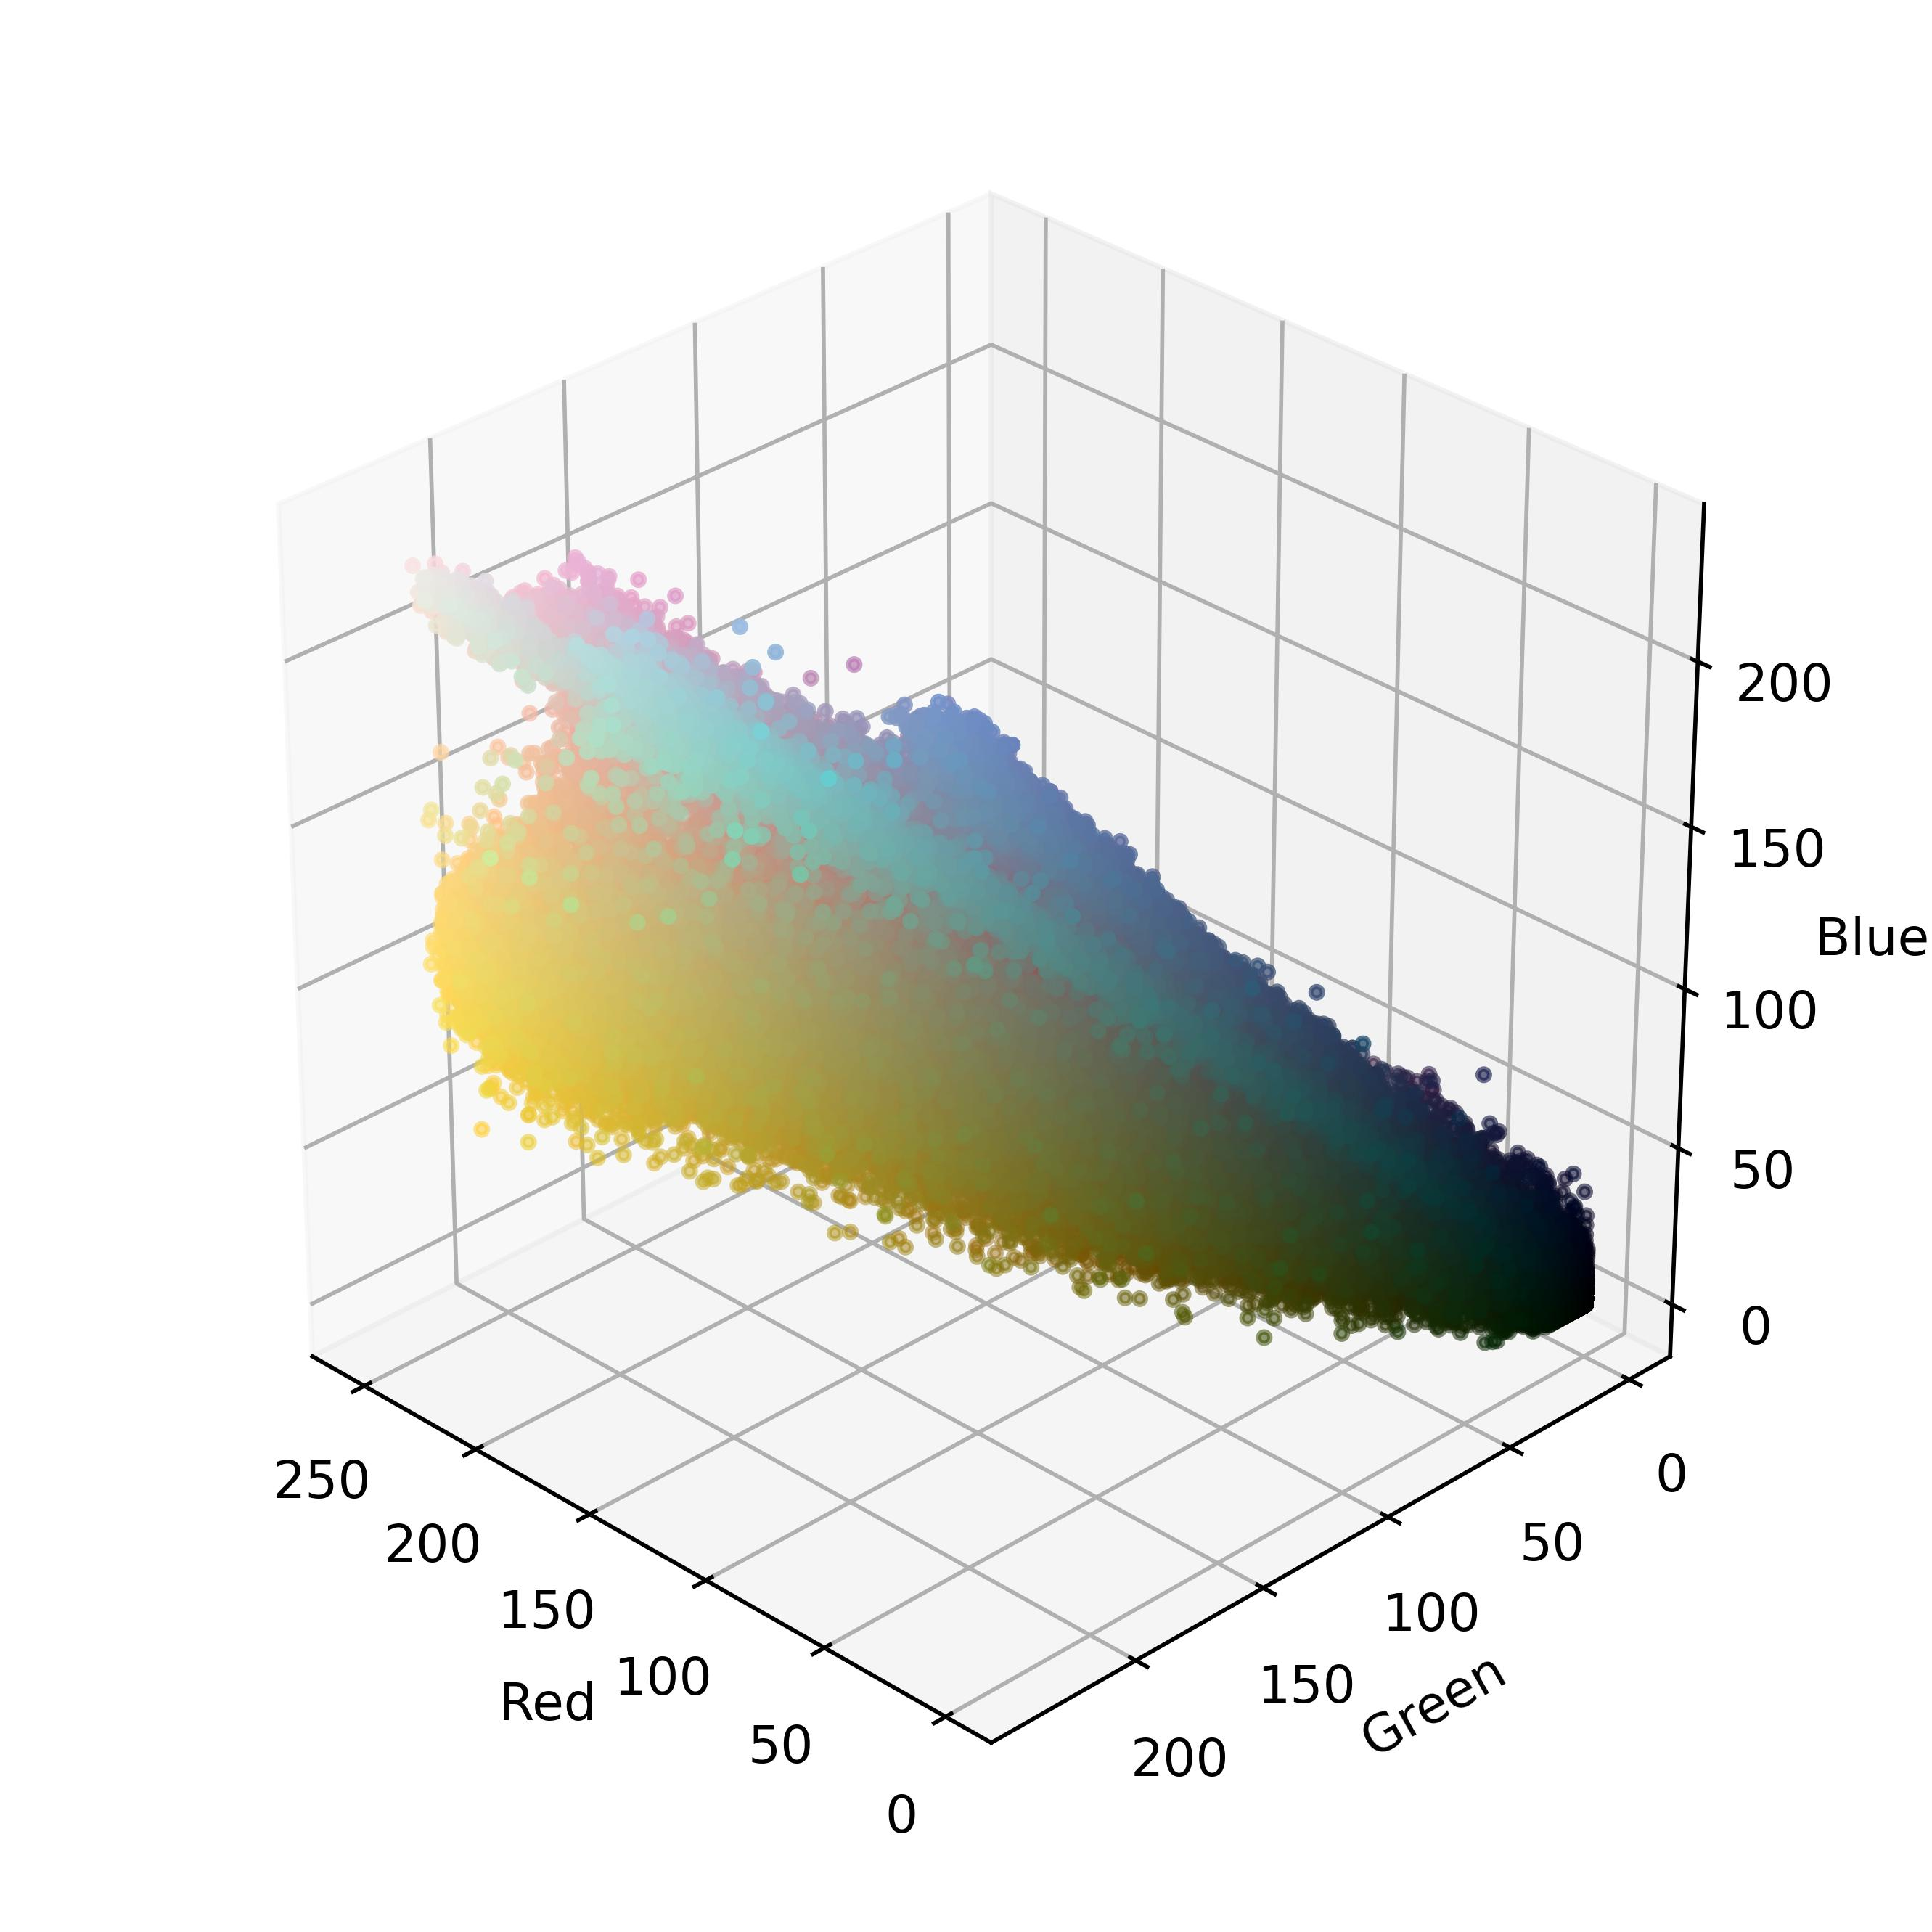
\includegraphics[width=\textwidth]{main_files/figure-latex/4_2_orange_marilyn_original_scatter.jpg}
    \caption{Orange Marilyn RGB Space Angle 2}
    \label{fig:4_2_orange_marilyn_original_scatter}
  \end{subfigure}
  \hfill
  \begin{subfigure}{0.24\textwidth}
    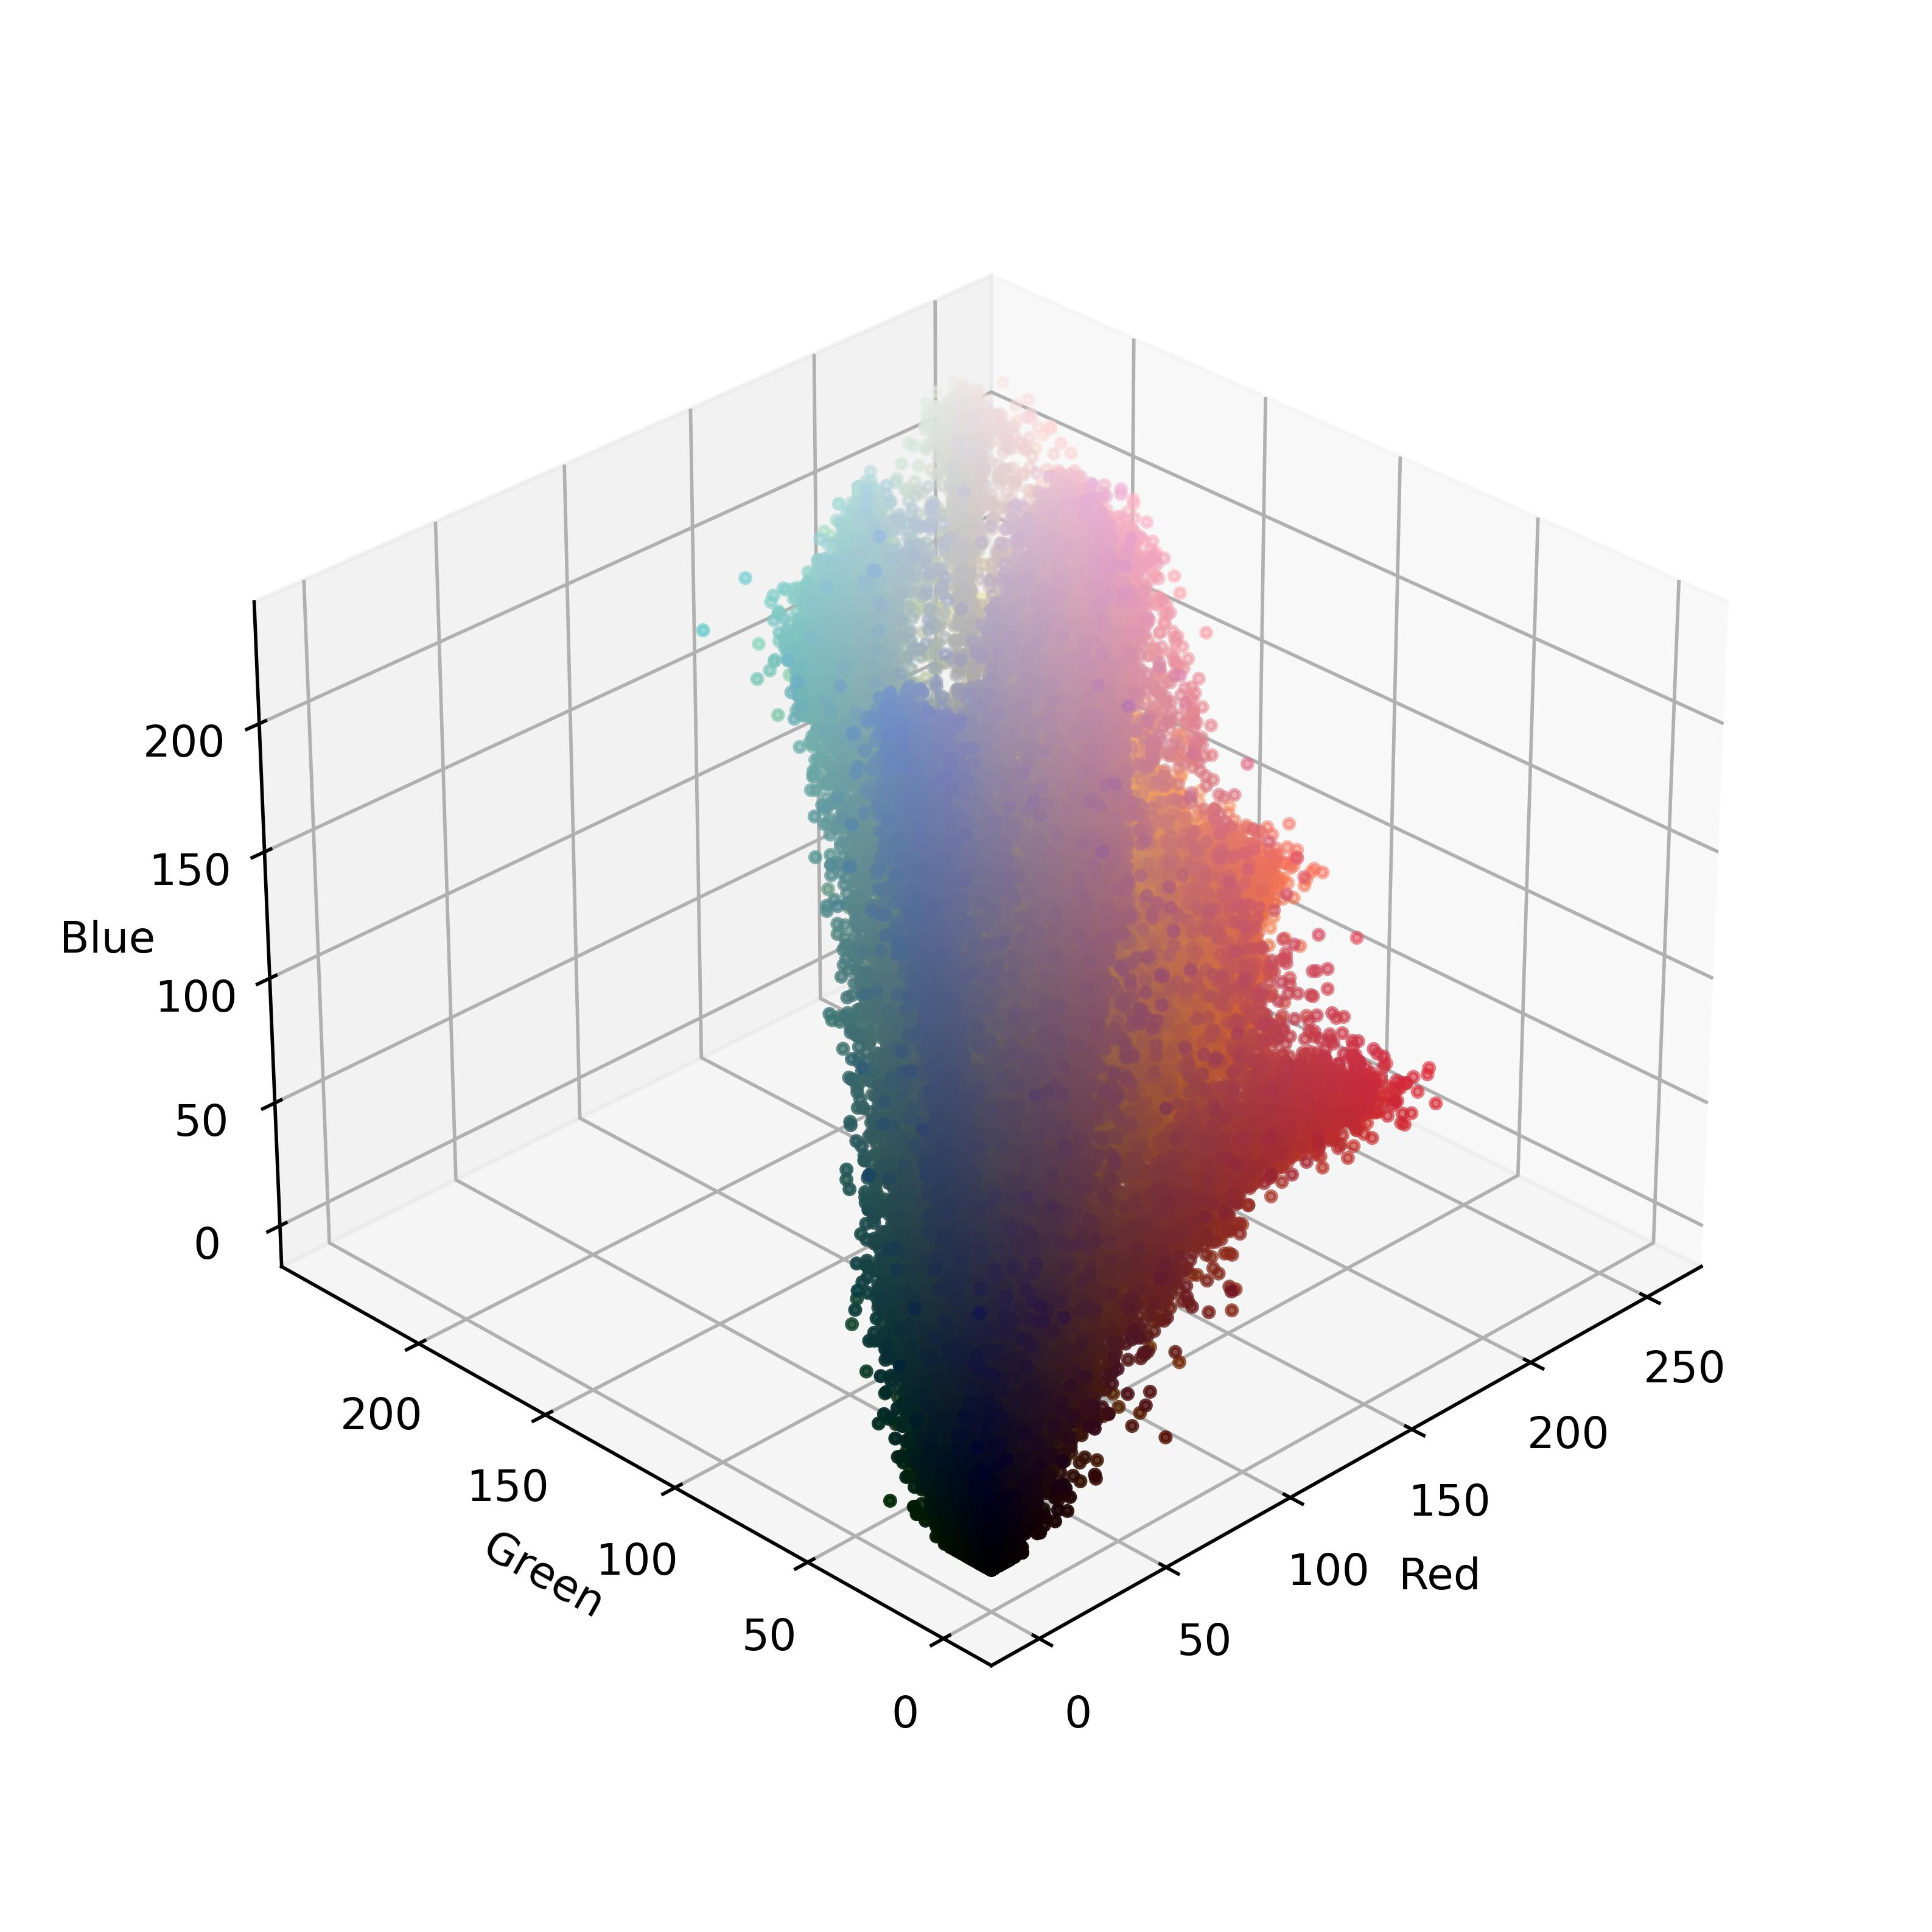
\includegraphics[width=\textwidth]{main_files/figure-latex/4_3_orange_marilyn_original_scatter.jpg}
    \caption{Orange Marilyn RGB Space Angle 3}
    \label{fig:4_3_orange_marilyn_original_scatter}
  \end{subfigure}
  \hfill
  \begin{subfigure}{0.24\textwidth}
    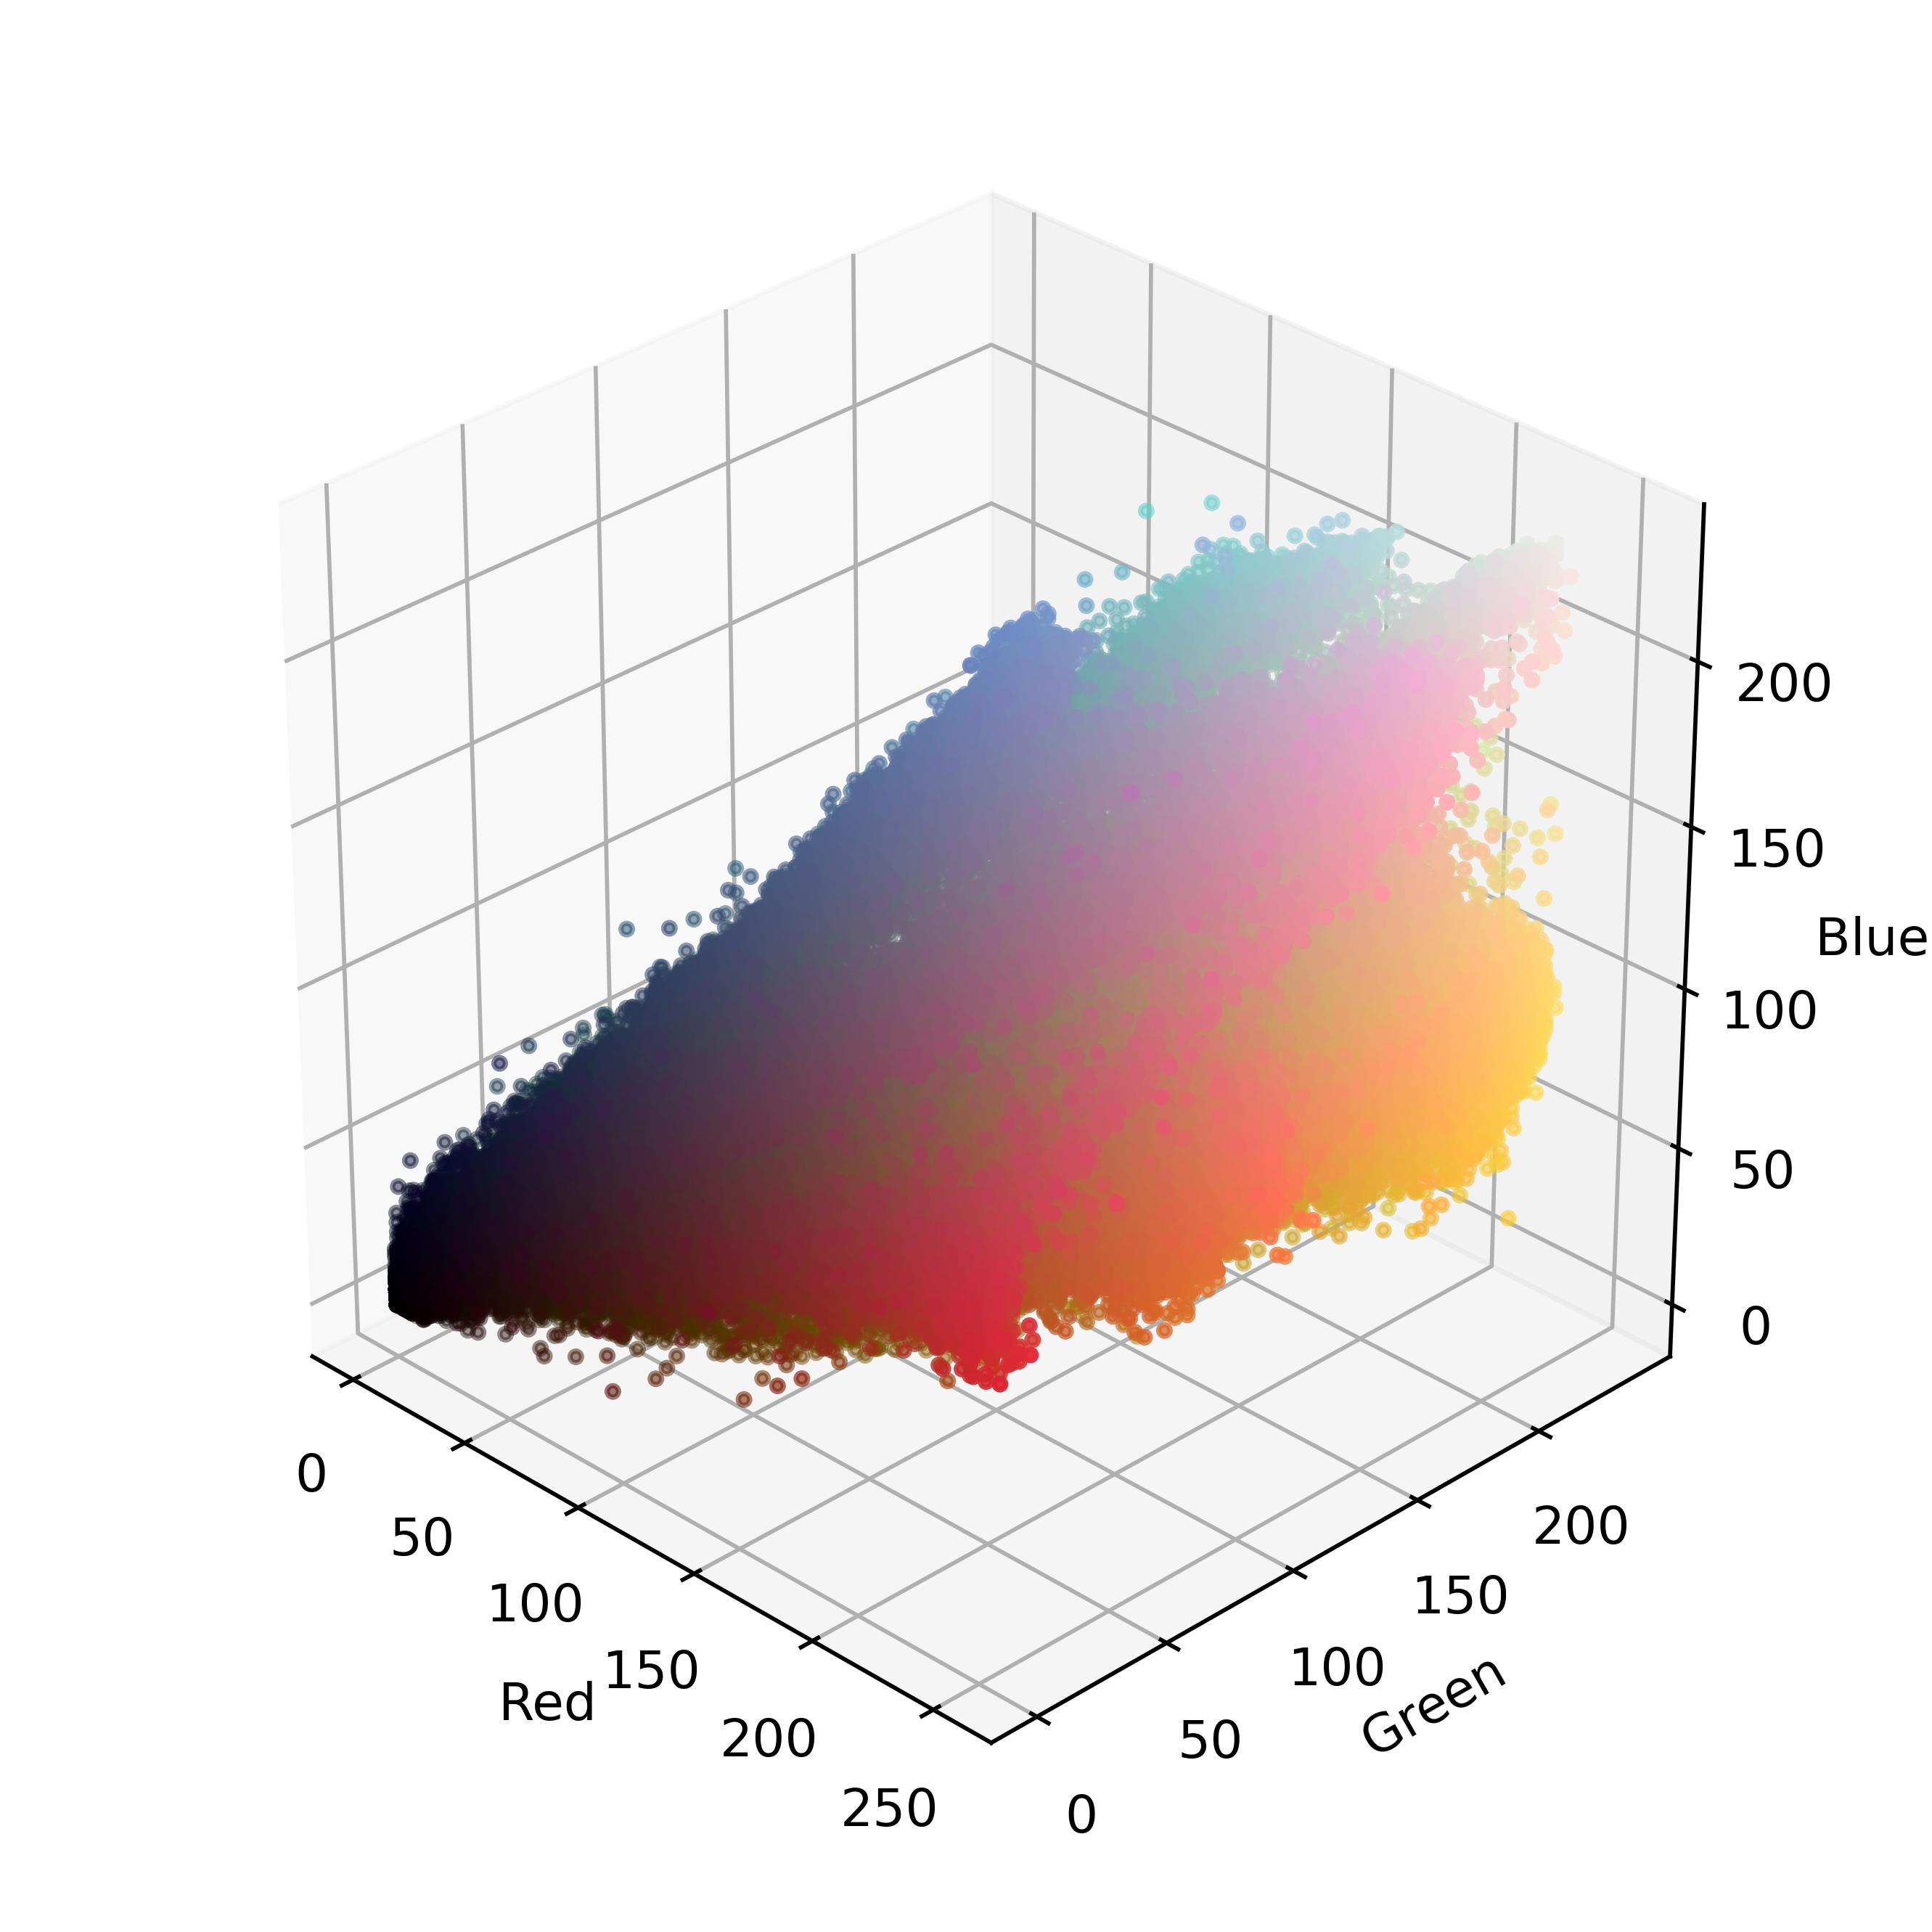
\includegraphics[width=\textwidth]{main_files/figure-latex/4_4_orange_marilyn_original_scatter.jpg}
    \caption{Orange Marilyn RGB Space Angle 4}
    \label{fig:4_4_orange_marilyn_original_scatter}
  \end{subfigure}
  \caption{The RGB space occupied by the pixels for the entire image of Orange Marilyn}
  \label{fig:orange_marilyn_scatter}
\end{figure}

Figure 4 displays the RGB space occupied by the pixels of the entire
image of Orange Marilyn from four different angles. Each subplot reveals
the distribution and density of pixel colors in the 3D RGB color space.
In (a), we observe a concentrated cluster of colors, indicating a
dominant presence of certain hues. In (b), the distribution spreads more
horizontally, highlighting the range of green and blue values. Plot (c)
shows a vertical spread, emphasizing the interplay between red and blue,
while (d) combines these perspectives, showcasing a broader color
distribution and illustrating the complex color dynamics present in the
image. These multiple viewpoints allow for a comprehensive understanding
of the color relationships within the artwork.

The following is a reference to the whole figure above, type this in
.Rmd:

\texttt{Figure\ \textbackslash{}ref\{fig:orange\_marilyn\_scatter\}}

It will show as:

Figure \ref{fig:orange_marilyn_scatter}

To reference a subplot:

\texttt{Figure\ \textbackslash{}ref\{fig:4\_2\_orange\_marilyn\_original\_scatter\}}

It will show as:

Figure \ref{fig:4_2_orange_marilyn_original_scatter}

\begin{figure}[ht]
  \centering
  \begin{subfigure}{0.24\textwidth}
    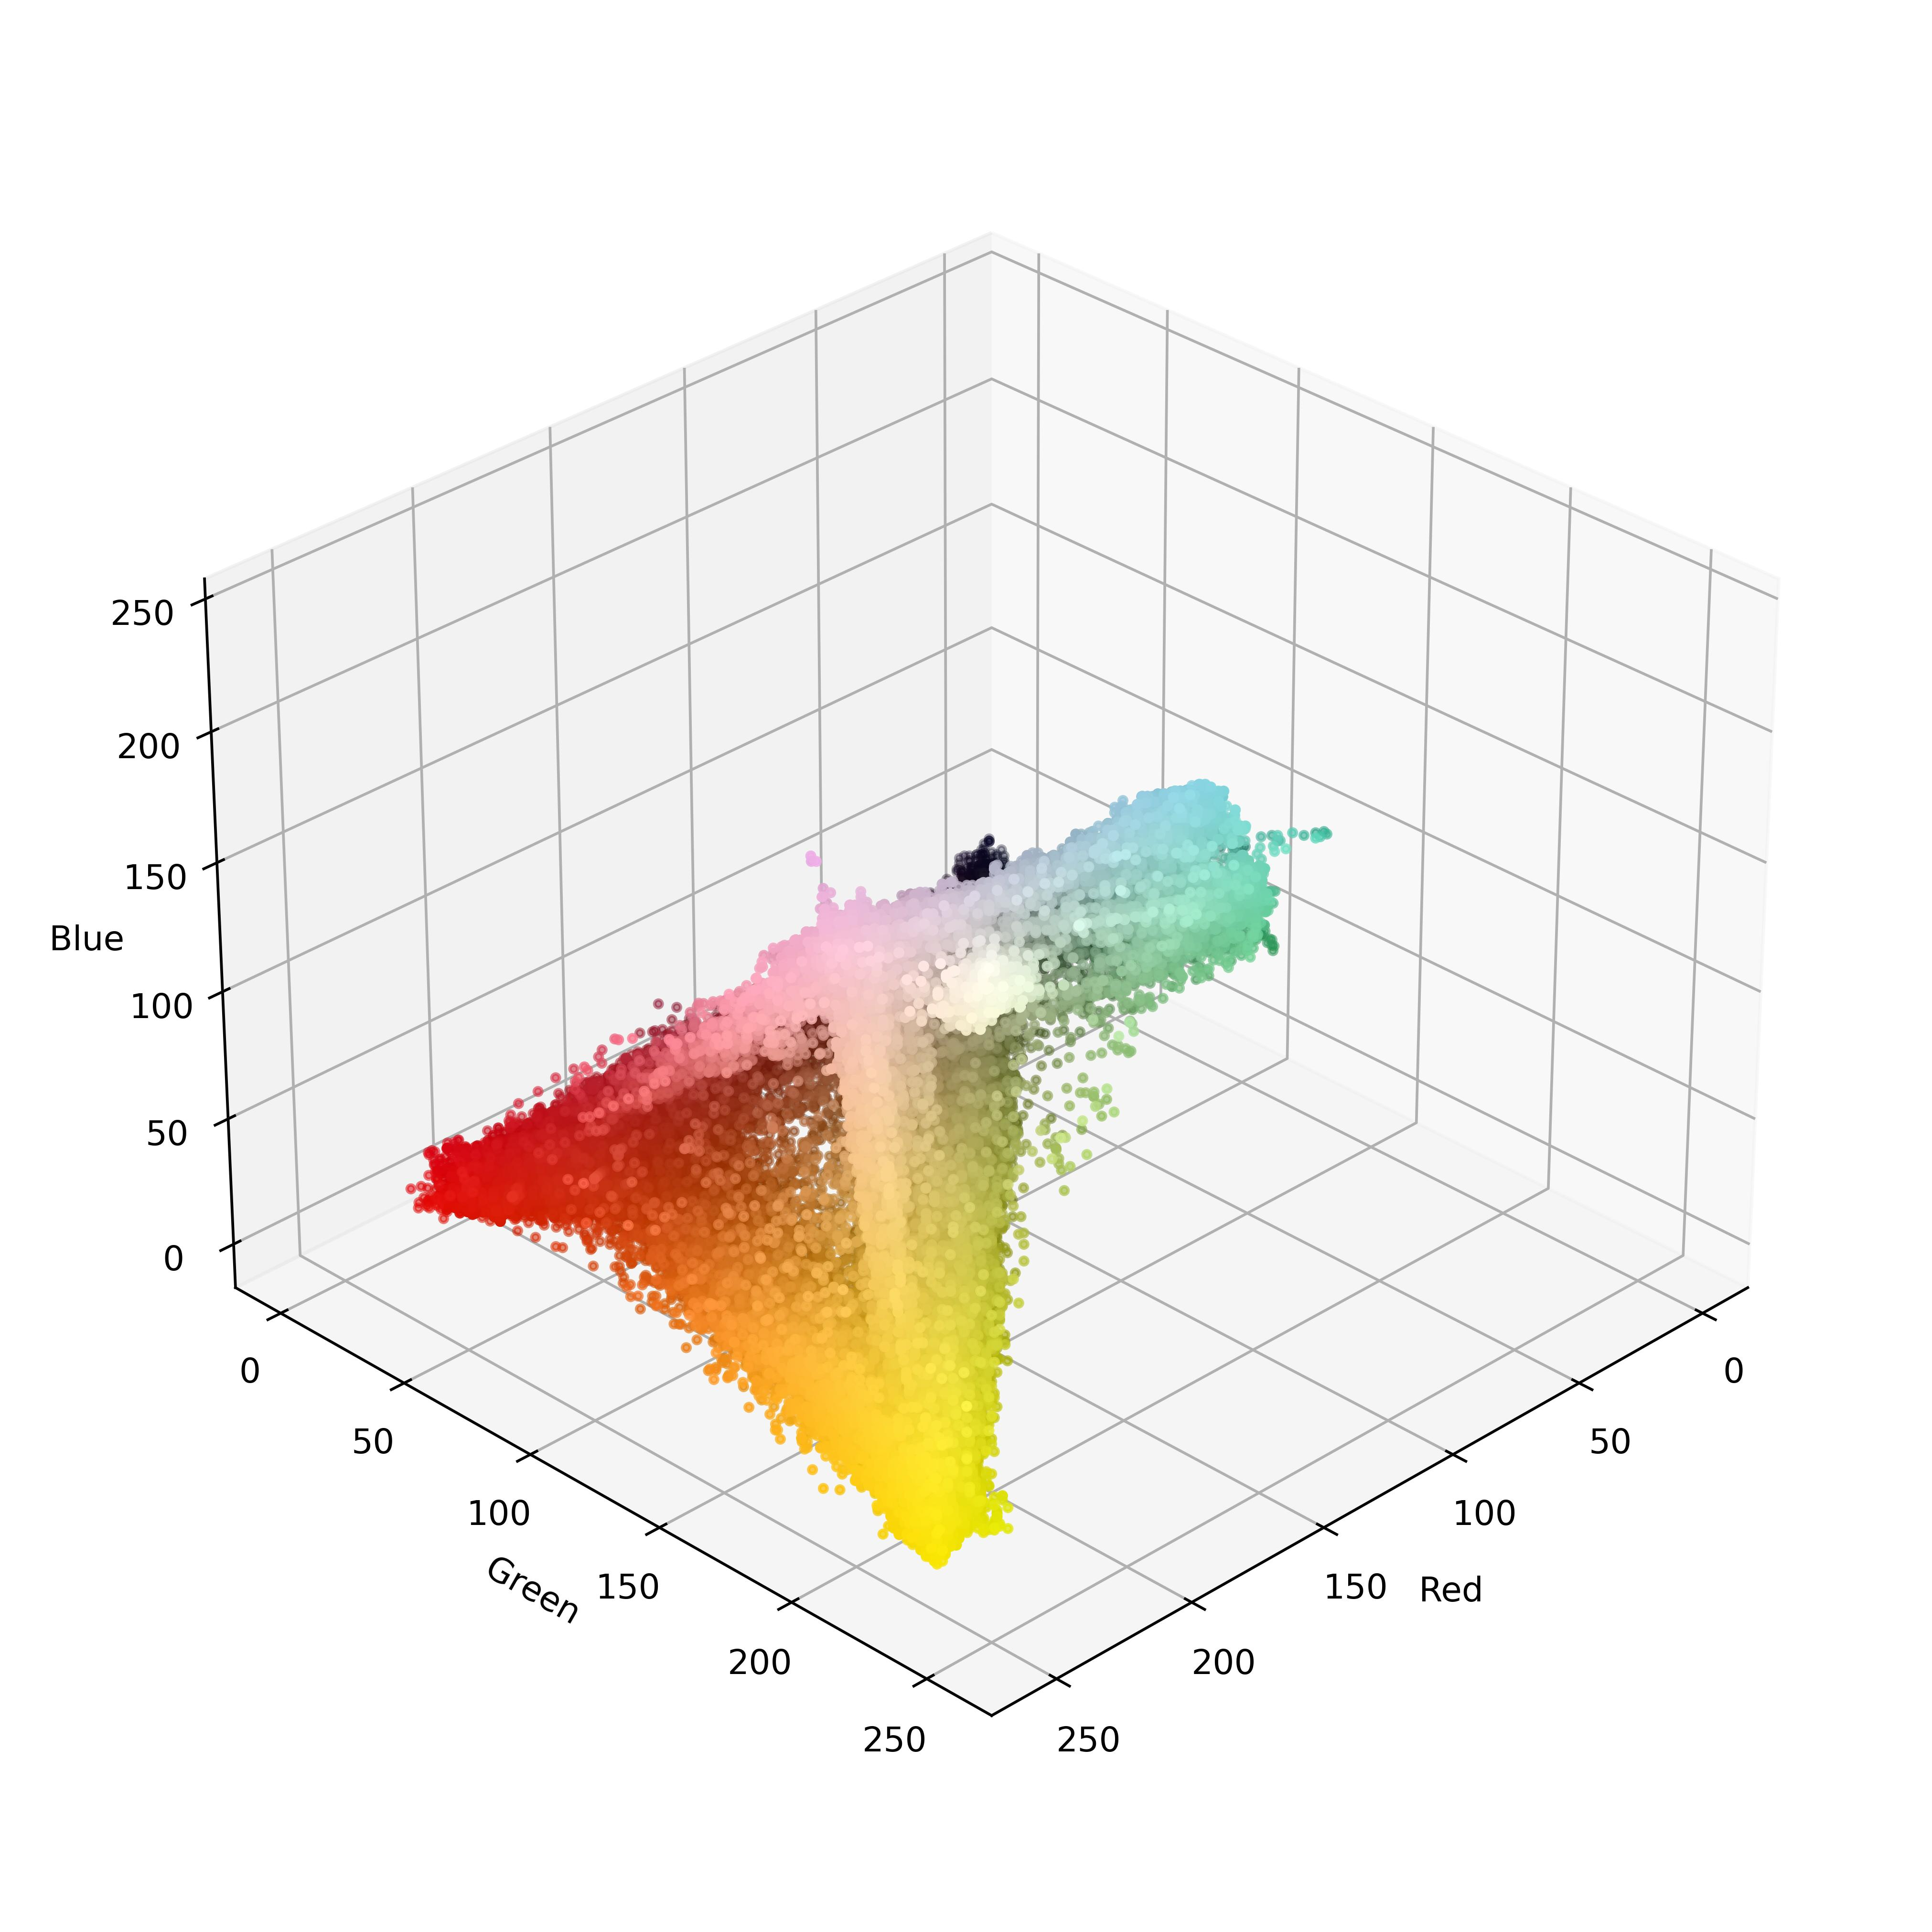
\includegraphics[width=\textwidth]{main_files/figure-latex/4_5_red_marilyn_original_scatter.jpg}
    \caption{Red Marilyn RGB Space Angle 1}
    \label{fig:4_5_red_marilyn_original_scatter}
  \end{subfigure}
  \hfill
  \begin{subfigure}{0.24\textwidth}
    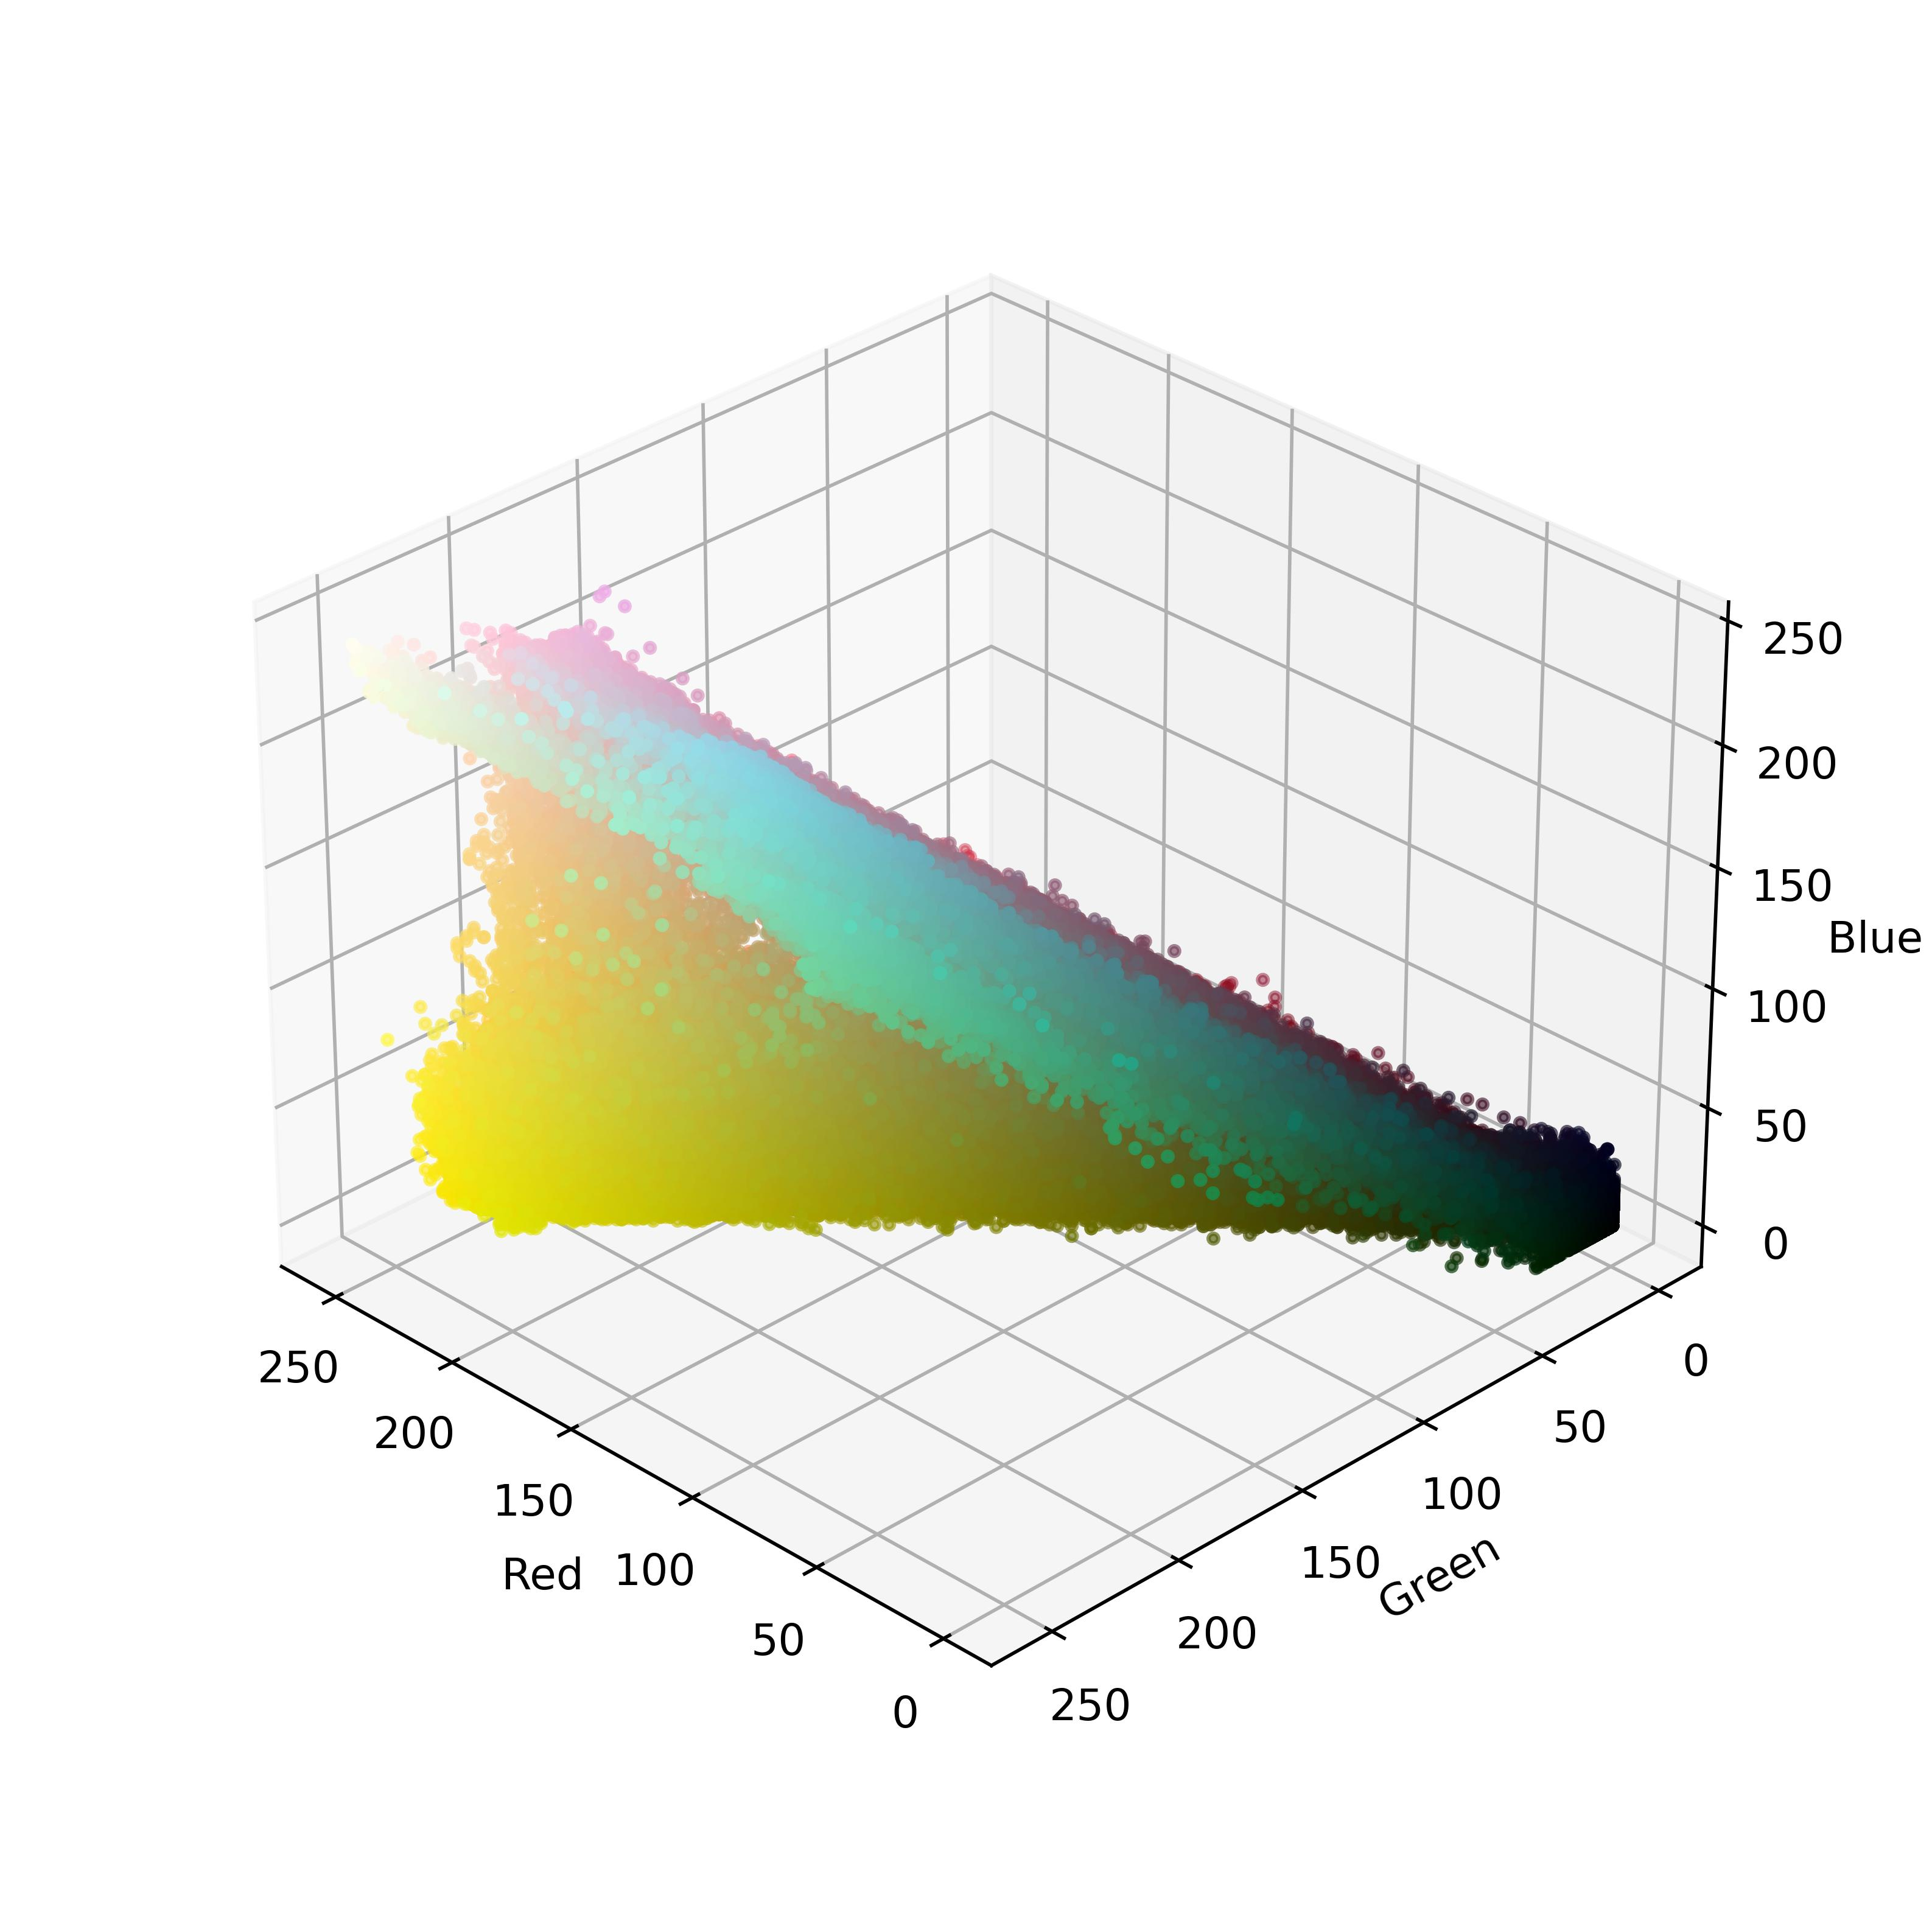
\includegraphics[width=\textwidth]{main_files/figure-latex/4_6_red_marilyn_original_scatter.jpg}
    \caption{Red Marilyn RGB Space Angle 2}
    \label{fig:4_6_red_marilyn_original_scatter}
  \end{subfigure}
  \hfill
  \begin{subfigure}{0.24\textwidth}
    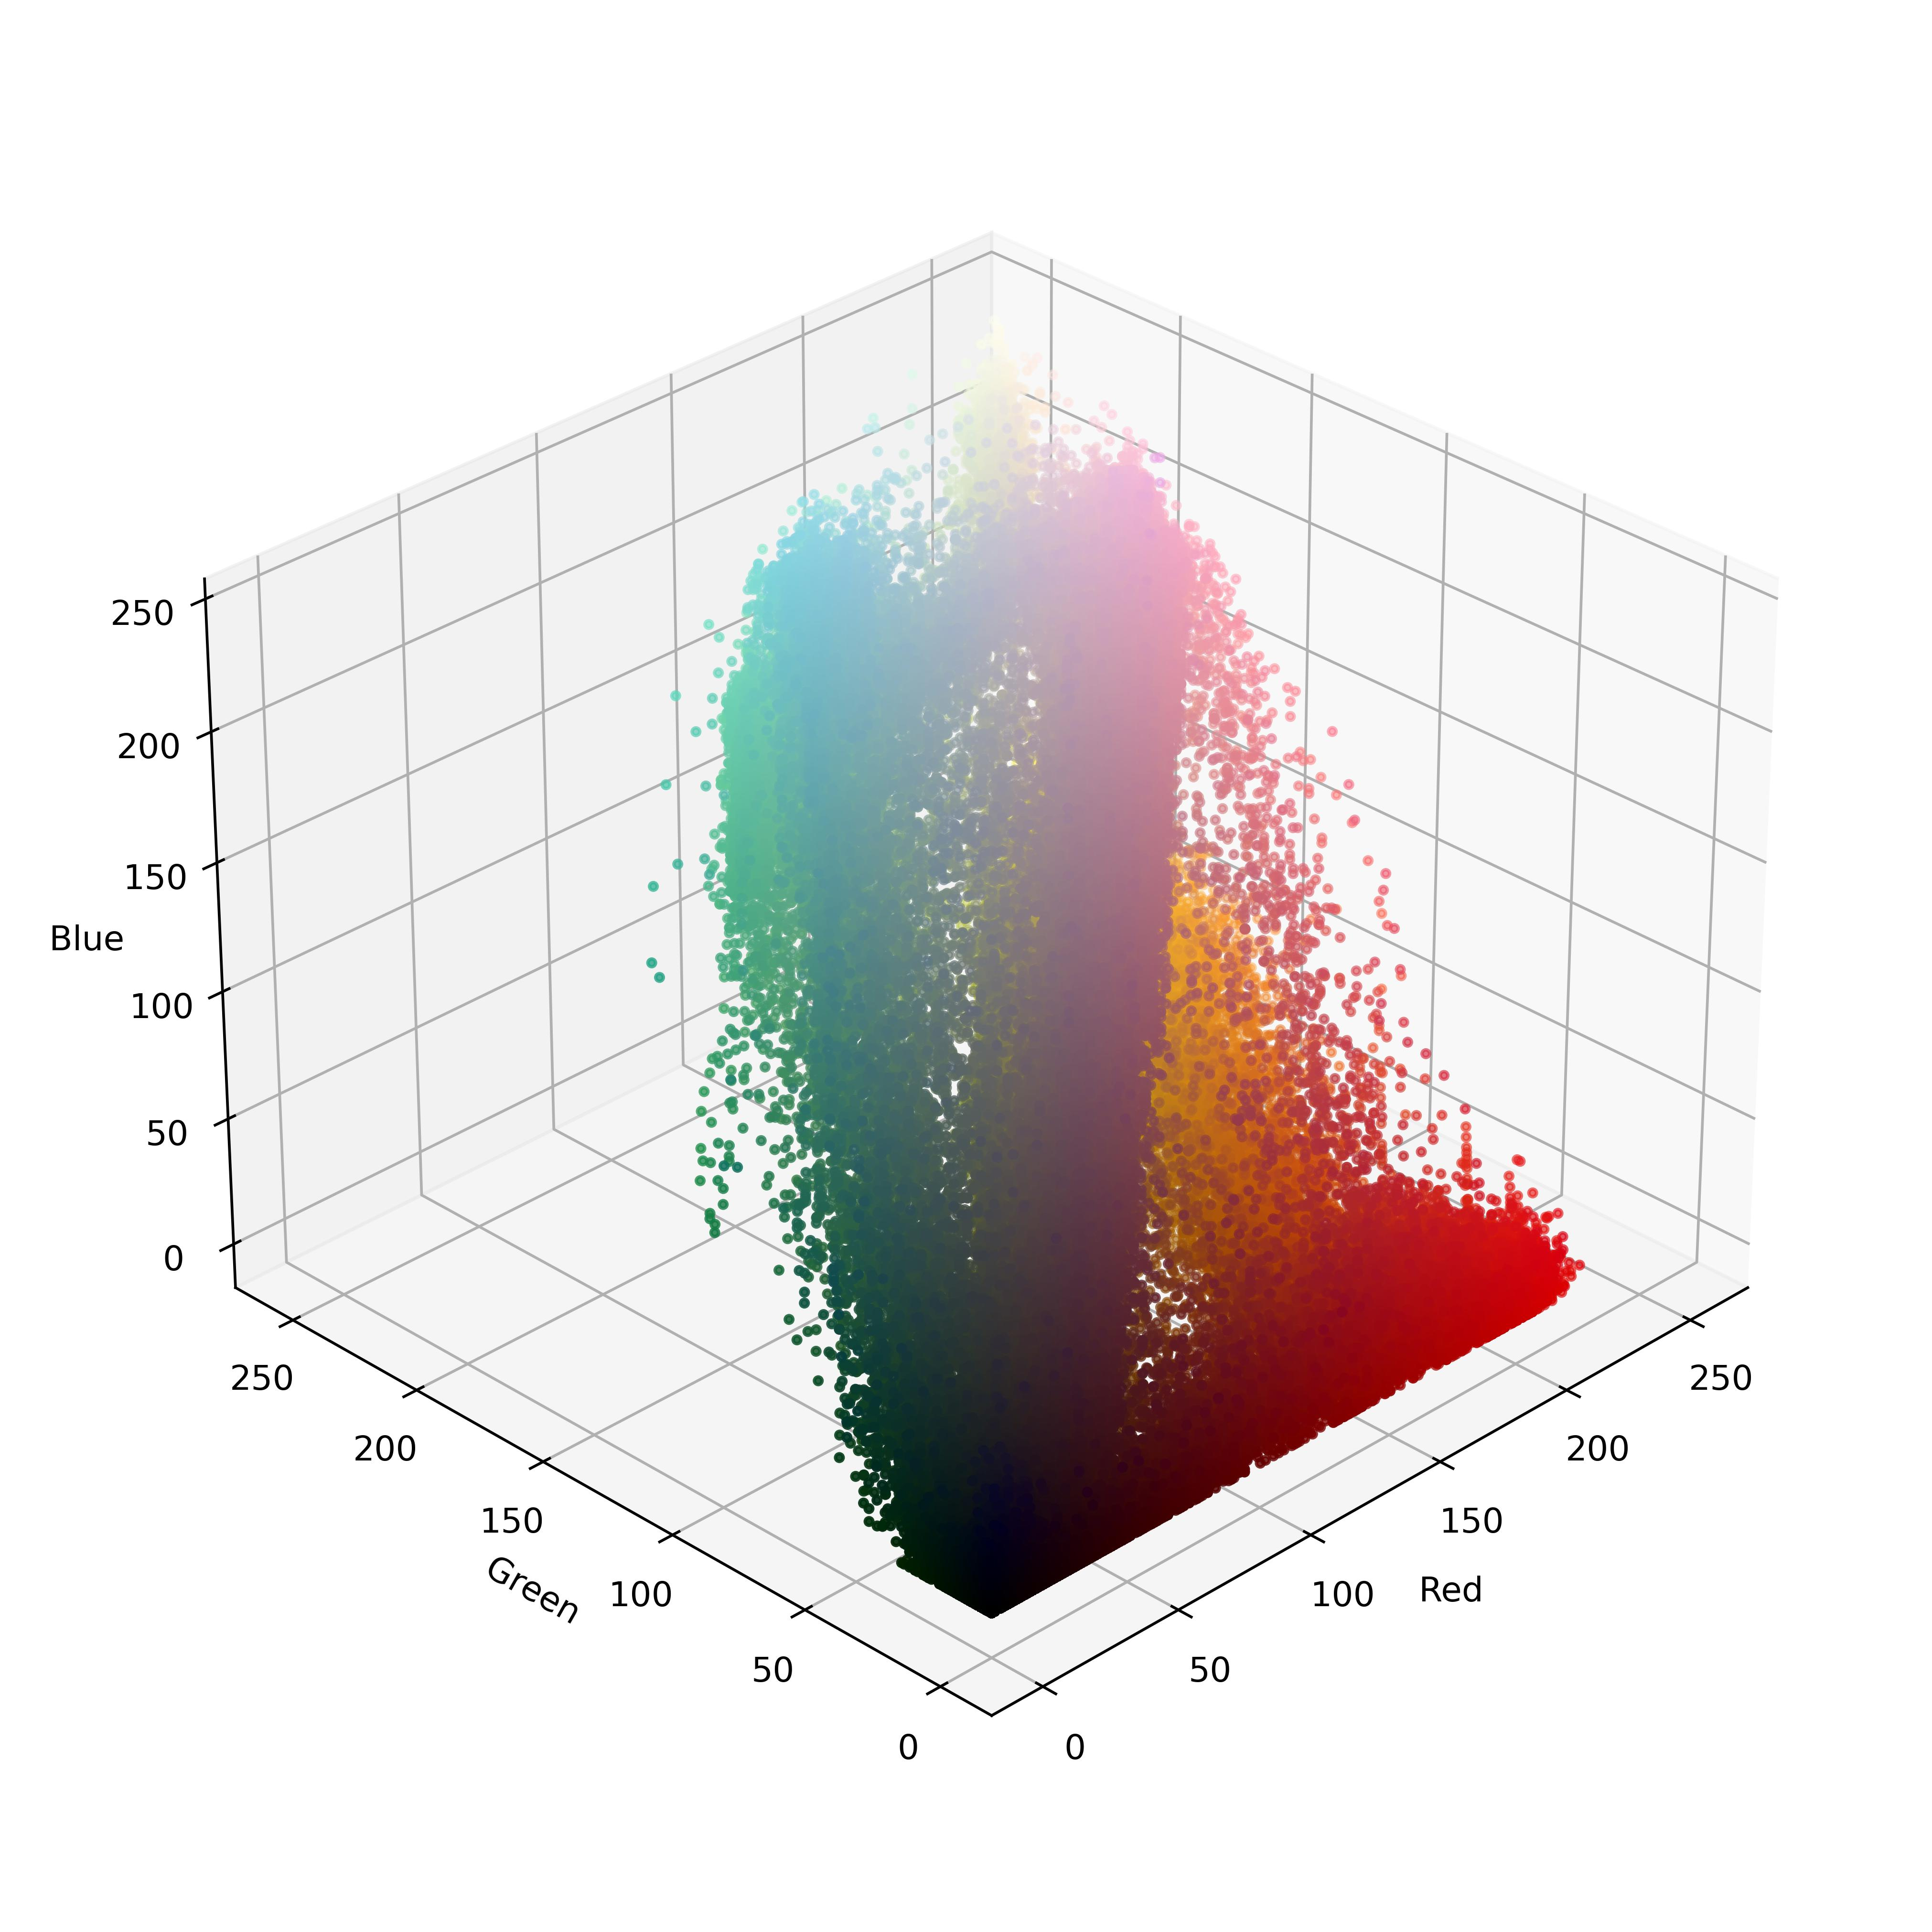
\includegraphics[width=\textwidth]{main_files/figure-latex/4_7_red_marilyn_original_scatter.jpg}
    \caption{Red Marilyn RGB Space Angle 3}
    \label{fig:4_7_red_marilyn_original_scatter}
  \end{subfigure}
  \hfill
  \begin{subfigure}{0.24\textwidth}
    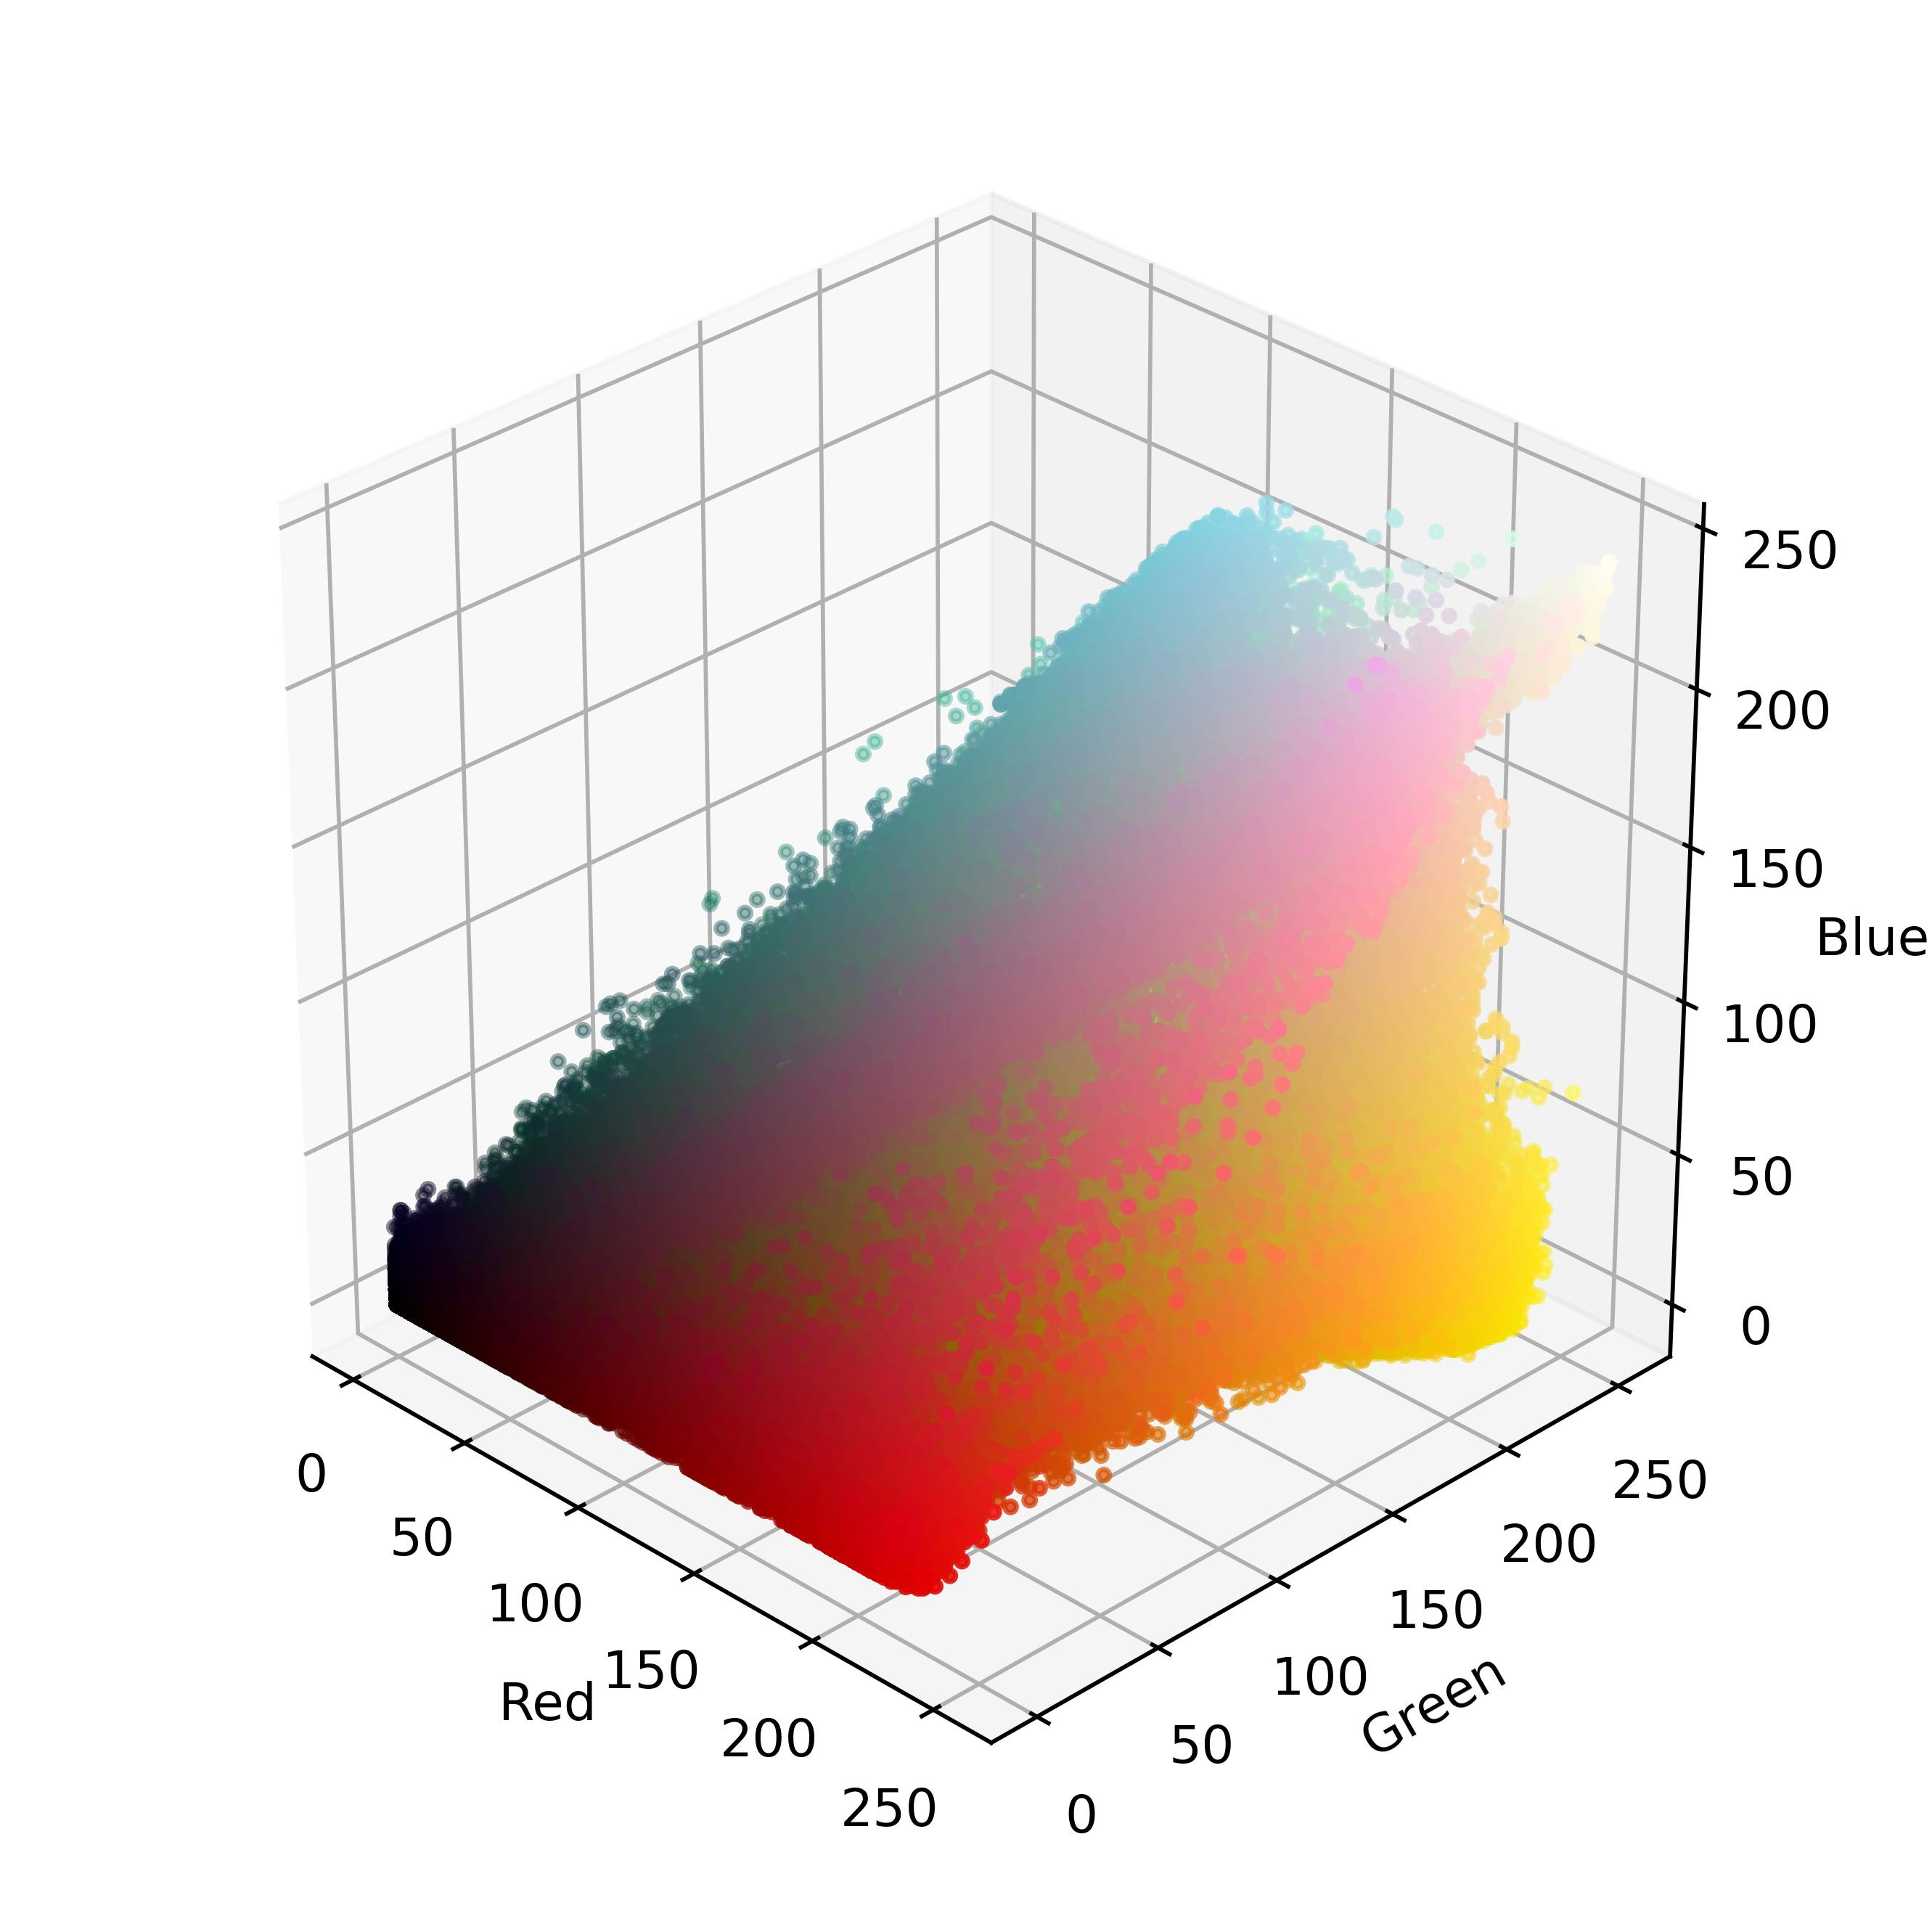
\includegraphics[width=\textwidth]{main_files/figure-latex/4_8_red_marilyn_original_scatter.jpg}
    \caption{Red Marilyn RGB Space Angle 4}
    \label{fig:4_8_red_marilyn_original_scatter}
  \end{subfigure}
  \caption{The RGB space occupied by the pixels for the entire image of Red Marilyn}
  \label{fig:red_marilyn_scatter}
\end{figure}

The following is a reference to the whole figure above, type this in
.Rmd:

\texttt{Figure\ \textbackslash{}ref\{fig:red\_marilyn\_scatter\}}

It will show as:

Figure \ref{fig:red_marilyn_scatter}

To reference a subplot:

\texttt{Figure\ \textbackslash{}ref\{fig:4\_7\_red\_marilyn\_original\_scatter\}}

It will show as:

Figure \ref{fig:4_7_red_marilyn_original_scatter}

\hypertarget{clustering-based-on-region-of-interest-roi}{%
\section{Clustering based on Region of Interest
(ROI)}\label{clustering-based-on-region-of-interest-roi}}

\hypertarget{repair-gunshot-of-image}{%
\section{Repair Gunshot of Image}\label{repair-gunshot-of-image}}

\hypertarget{disuccsion}{%
\section{Disuccsion}\label{disuccsion}}

\hypertarget{conclusion-and-future-work}{%
\section{Conclusion and Future Work}\label{conclusion-and-future-work}}

\bibliographystyle{unsrt}
\bibliography{references.bib}


\end{document}
